\documentclass[utf8, smaller, c]{beamer}
	\usepackage[mnf, foottitle]{citlab/beamerthemeCITlab}
	\usepackage{citlab/CITlab}
	\usepackage{citlab/CITlab_JM}
% 	\usepackage[utf8]{inputenc}
%   \usepackage[T1]{fontenc}
	\usepackage{lmodern}
	
	\usepackage{url}
	\usepackage{caption}
    \renewcommand{\figurename}{Abbildung}
    % \usepackage{hyperref}
    \usepackage{listings}
    \lstset{language=python, basicstyle=\footnotesize, tabsize=4, columns=fullflexible, xleftmargin=\parindent}
    \renewcommand{\tt}[1]{{\texttt{#1}}}
	
\begin{document}

	\author{M.Sc.~Johannes~Michael}
    \institute[Uni Rostock]{Universität Rostock}
	\date[05.~November~2021]{Johannes Michael}
	\title{Mathematisches Praktikum}
	\subtitle{Grundlagen TensorFlow}

	\setbeamertemplate{footline}{\usebeamertemplate{firstFootline}}
	\frame{\maketitle}

	\setbeamertemplate{caption}{\insertcaption}
	\setbeamertemplate{footline}{\usebeamertemplate{allFootline}}

    \setbeamertemplate{section in toc}[ball unnumbered]
    \setbeamertemplate{subsection in toc}[square]
 	\frame{\tableofcontents}

%%%%%%%%%%%%%%%%%%%%
\section{TensorFlow}
%%%%%%%%%%%%%%%%%%%%
\begin{frame}[fragile]{TensorFlow}
	\begin{itemize}
		\item Plattformunabhängige Open-Source-Programmbibliothek für maschinelles Lernen von Google
			\item Kanonische import-Anweisung in Python:
	\begin{lstlisting}
import tensorflow as tf
	\end{lstlisting}
        \item Unterstützt numerische Berechnungen unter Verwendung von Datenflussgraphen	
	    \item Kernelement für Daten in TensorFlow: \textbf{Tensor} ($n$-dim. array)
	\end{itemize}
\end{frame}

%%%%%%%%%%%%%%%%%%
\section{Tensoren}
%%%%%%%%%%%%%%%%%%
\begin{frame}[fragile]{Tensoren}
	\begin{itemize}
		\item Tensoren sind immutable (Ausnahme: \tt{tf.Variable}).
		\item \textbf{Rang} (rank) und \textbf{Form} (shape) eines Tensors analog zu NumPy arrays
	\end{itemize}
	{\small
	\begin{center}
	\begin{tabular}{c|l|l|l}
		Tensor & Rank & Shape & Bemerkung \\ \hline
		$2$ & 0 & [] & Skalar \\
		$[1, 2]$ & 1 & [2] & Vektor \\
		$[[1, 2]$, $[3, 4]]$ & 2 & [2, 2] & Matrix \\
		$[[[1, 2], [3, 4]],\,[[5, 6], [7, 8]]]$ & 3 & [2, 2, 2] &  3-dim. Array
	\end{tabular}
	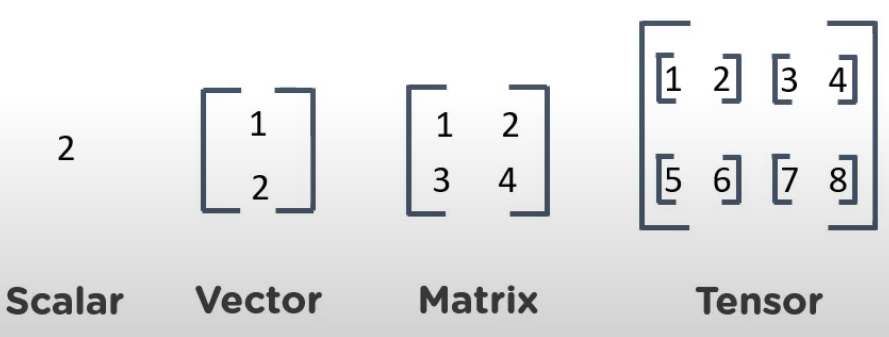
\includegraphics[scale=0.2]{pics/tensors}\\
	{\tiny Source: "TensorFlow 2.0 Tutorial for Beginners" (\url{youtube.com/watch?v=QPDsEtUK_D4})}
	\end{center}
	}
\end{frame}

%%%%%%%%%%%%%%%%%%%%%%%%%%
\section{Berechnungsgraph}
%%%%%%%%%%%%%%%%%%%%%%%%%%
\begin{frame}[fragile, allowframebreaks]{Berechnungsgraph}
	\begin{itemize}
		\item Klassische TensorFlow Programme bestehen aus 2 Phasen:
		\begin{itemize}
			\item[1)] Erzeugung des Berechnungsgraphen.
			\item[2)] Ausführung des Berechnungsgraphen.
		\end{itemize}
		% $\rightarrow$ verzögerte Ausführung des Programmcodes.
		\item Der \textbf{Berechnungsgraph} (computational graph) bildet ein Netz von Knoten, die über Kanten verbunden werden und repräsentiert Berechnungen als Abhängigkeiten zwischen individuellen Operationen.
		\begin{itemize}
			\item Knoten: TensorFlow Operationen (\textit{ops}) mit $n \geq 0$ Eingabetensoren und $1$ Ausgabetensor.
			\item Kanten: Datenfluss über Tensoren.
		\end{itemize}
	\end{itemize}
	
	\framebreak
	
	\begin{itemize}
	    \item Berechne folgende Funktion:\\[-3mm]
	\end{itemize}
	\begin{align*}
	    a(b,c,d)=(b+c)*(d-4)
	\end{align*}
	\vspace*{-8mm}
	\begin{itemize}
	    \item Zugehöriger Datenflussgraph:
	\end{itemize}
	\begin{center}
	    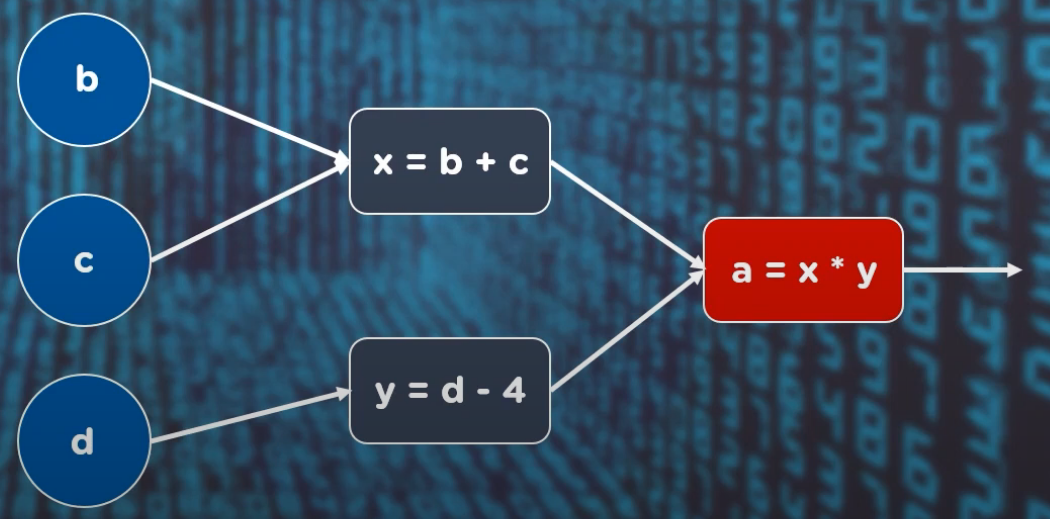
\includegraphics[scale=0.2]{pics/datagraph_example.png}\\
	    {\tiny Source: "TensorFlow 2.0 Tutorial for Beginners" (\url{youtube.com/watch?v=QPDsEtUK_D4})}
	\end{center}
	
	\framebreak
	
	\begin{itemize}
		\item Warum Datenflussgraphen?
		\begin{itemize}
			\item \textbf{Parallelität:} Kanten im Graph repräsentieren Abhängigkeiten zwischen Operationen $\rightarrow$ Das System kann Operationen identifizieren die parallel ausgeführt werden können.
			\item \textbf{Verteilte Ausführung:} TensorFlow kann das Programm über mehrere Geräte (CPUs, GPUs) verteilen und die nötige Koordination selbstständig hinzufügen.
			\item \textbf{Kompilieren:} TensorFlows XLA compiler kann den Datenflussgraph optimieren (z.B. Operationen verschmelzen).
			\item \textbf{Portierbarkeit:} Datenflussgraph ist sprachen-unabhängige Modelrepräsentation $\rightarrow$ In Python gebauter Graph kann gespeichert und in Java geladen werden.
		\end{itemize}
	\end{itemize}
\end{frame}

%%%%%%%%%%%%%%%%%%%%%%%%%%%%%%%
\section{TensorFlow 1.x vs 2.x}
%%%%%%%%%%%%%%%%%%%%%%%%%%%%%%%
\begin{frame}[fragile]{TensorFlow 1.0 vs 2.0}
    \begin{columns}
        \begin{column}{0.54\textwidth}
            \textbf{TensorFlow 1.x}
            \begin{itemize}
                \item Arbeitet \textit{nur} mit Datenflussgraphen
                \item[$\rightarrow$] Eingaben über \tt{tf.placeholder()}
                \item[$\rightarrow$] Auswertung über \tt{tf.Session()}
            \end{itemize}
            \begin{lstlisting}
    outputs = session.run(f(placeholder),
                feed_dict={placeholder:input})
            \end{lstlisting}
            \begin{itemize}
                \item Eingeschränkte Python Funktionen im Graphmodus
            \end{itemize}
        \end{column}
        \begin{column}{0.46\textwidth}
            \textbf{TensorFlow 2.x}
            \begin{itemize}
                \item Unterstützt standardmäßig \textit{eager execution}
            \end{itemize}
            \begin{lstlisting}
    outputs = f(input)
            \end{lstlisting}
            \begin{itemize}
                \item \tt{tf.function()} decorator lässt Python Funktionen im Graphmodus laufen
                \item[$\rightarrow$] \textit{AutoGraph} feature wandelt Python Code automatisch in TensorFlow ops um
            \end{itemize}
        \end{column}
    \end{columns}
\end{frame}

%%%%%%%%%%%%%%%%%%%%%%%%%%%%%%%%%%%%%%%%%%
\section{TensorFlow 2.0 Toolkits Hierarchie}
%%%%%%%%%%%%%%%%%%%%%%%%%%%%%%%%%%%%%%%%%%
\begin{frame}[fragile]{TensorFlow 2 Toolkits Hierarchie}
    \begin{center}
        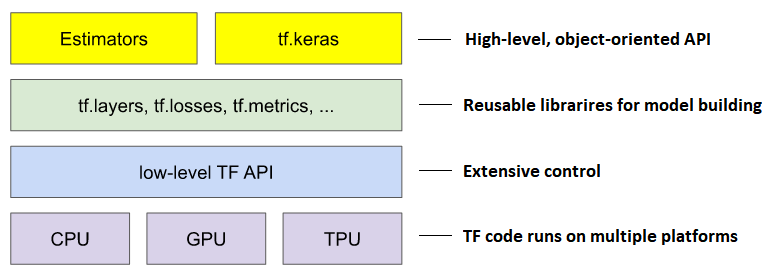
\includegraphics[scale=0.5]{pics/tf_hierarchy}\\
        {\tiny Source: \url{developers.google.com/machine-learning/crash-course/first-steps-with-tensorflow/toolkit}}
    \end{center}
    \begin{itemize}
        \item \tt{tf.keras} ist die offizielle high-level API von TensorFlow 2.0
        \item[$\rightarrow$] Stellt mehrere APIs zum Bauen von Modellen zur Verfügung (\textit{Sequential}, \textit{Functional}, \textit{Subclassing})
    \end{itemize}
\end{frame}

%%%%%%%%%%%%%%%%%%%%%%%
\section{Tensor--Basics}
%%%%%%%%%%%%%%%%%%%%%%%
\begin{frame}[fragile, allowframebreaks]{Tensor--Basics}
	\begin{itemize}
		\item \tt{tf.constant(value, dtype=None, shape=None)}\\(intern gespeicherter, unveränderlicher Tensor)
		\item Standardops $+,-,*,/$ in TensorFlow überladen, unterstützen Broadcasting, erwarten passende dtypes\\(\tt{tf.add}, \tt{tf.subtract}, \tt{tf.multiply}, \tt{tf.divide})
	\begin{lstlisting}
	c1 = tf.constant(3.0)  # Skalar
    c2 = tf.constant(5.0)  # Skalar
    c3 = c1 + c2  # oder tf.add(c1, c2)
    c4 = c1 * c2  # oder tf.multiply(c1, c2)
    print(c1, c2, c3, c4, sep="\n")
	# tf.Tensor(3.0, shape=(), dtype=float32)
    # tf.Tensor(5.0, shape=(), dtype=float32)
    # tf.Tensor(8.0, shape=(), dtype=float32)
    # tf.Tensor(15.0, shape=(), dtype=float32)
	\end{lstlisting}
	\end{itemize}

    \framebreak
    
    \begin{itemize}
        \item Datentyp von Tensoren kann verändert werden
    \end{itemize}
    \begin{lstlisting}
    x = tf.constant([[8, 8], [6, 6]])  # int32
    x = tf.cast(x, dtype=tf.float32)  # float32
    \end{lstlisting}
    \begin{itemize}
        \item Diverse Tensor-Initialisierungen analog zu NumPy
    \end{itemize}
    \begin{lstlisting}
    tf.constant(list(range(1, 9)), shape=[4, 2])  # Shape-Umformung
    tf.ones(shape)  # Einsen
    tf.zeros(shape)  # Nullen
    tf.range(start, limit, delta)  # gleichverteilte Werte aus [start, limit), analog zu range()
    tf.linspace(start, stop, num)  # 'num' viele gleichverteilte Werte aus [start, stop]
    tf.random.uniform(shape, minval, maxval)  # Zufallswerte aus Gleichverteilung
    tf.random.normal(shape, mean, stddev)  # Zufallswerte aus Normalverteilung
    \end{lstlisting}
    $\dots$ und viele weitere (siehe {\footnotesize\url{tensorflow.org/api_docs/python/tf}}) 
    
    \framebreak

	\begin{itemize}
		\item \textbf{Variablen} repräsentieren Tensoren die zur Laufzeit veränderlich sind
		\item \tt{tf.Variable(initial\_value, dtype=None, shape=None)} 
		\begin{lstlisting}
	x = tf.Variable([[1, 2, 3]], name="x")
    print(x)  # <tf.Variable 'x:0' shape=(1, 3) dtype=int32, numpy=array([[1, 2, 3]])>
    x.assign(x + tf.ones_like(x))  # Variable neuen Wert zuweisen
    print(x)  # <tf.Variable 'x:0' shape=(1, 3) dtype=int32, numpy=array([[2, 3, 4]])>
		\end{lstlisting}
		\item TensorFlow Operationen verarbeiten Tensoren und Variablen gleichermaßen
		\begin{lstlisting}
	y = tf.ones([3, 3], dtype=tf.int32)
    z = tf.matmul(x, y)  # Matrixmultiplikation
    print(z)  # tf.Tensor([[9 9 9]], shape=(1, 3), dtype=int32)
		\end{lstlisting}
	\end{itemize}
	
	\framebreak
	
	\begin{itemize}
	    \item Kompatibilität zu NumPy arrays:
	    \begin{itemize}
	        \item TensorFlow Operationen konvertieren NumPy arrays zu Tensoren
	        \item NumPy Operationen konvertieren Tensoren zu NumPy arrays
	        \item Tensoren können explizit zu NumPy arrays umgewandelt werden
	    \end{itemize}
	\end{itemize}
	\begin{lstlisting}
    ndarray = np.ones([2, 3])
    tensor = tf.multiply(ndarray, 5)
    array = np.add(tensor, -3)
    print(tensor)  # tf.Tensor([[5. 5. 5.]], shape=(1, 3), dtype=float64)
    print(array, type(array))  # [[2. 2. 2.]] <class 'numpy.ndarray'>
    print(tensor.numpy(), type(tensor.numpy()))  # [[5. 5. 5.]] <class 'numpy.ndarray'>
	\end{lstlisting}
	\begin{itemize}
	    \item Indizieren und Slicen analog zu NumPy arrays
	    \item[$\rightarrow$] [start:stop:step] für jede Dimension des Tensors
	\end{itemize}
\end{frame}

%%%%%%%%%%%%%%%%%%%%%%%%%%%%%%%%%
\section{Tensor--Transformationen}
%%%%%%%%%%%%%%%%%%%%%%%%%%%%%%%%%
\begin{frame}[fragile, allowframebreaks]{Tensor--Transformationen}
	\begin{itemize}
		\item \tt{tf.reshape(tensor, shape)}:\\Umformung der Dimensionen
		\begin{lstlisting}
	tensor = tf.constant(2.0, shape=[28, 28])
    t1 = tf.reshape(tensor, [14, 56])
    t2 = tf.reshape(tensor, [-1, 2])  # -1 entspricht "restlicher" shape
    t3 = tf.reshape(tensor, [28, 14, 2])
    t4 = tf.reshape(tensor, [28, 1, 28])
		\end{lstlisting}
		\item \tt{tf.expand\textunderscore dims(tensor, dim)}:\\Hinzufügen einer 1-Dimension
		\begin{lstlisting}
	tensor = tf.constant(2.0, shape=[28, 28])
    t_expand = tf.expand_dims(tensor, axis=1)  # (28, 1, 28)
		\end{lstlisting}
		\item \tt{tf.squeeze(tensor, dim)}:\\Löschen einer (aller) 1-Dimension(en)
		\begin{lstlisting}
	tensor = tf.constant(2.0, shape=[28, 1, 1, 28, 1])
    t_squeeze = tf.squeeze(tensor, 1)  # (28, 1, 28, 1)
    t_squeeze_2 = tf.squeeze(t_squeeze)  # (28, 28)
		\end{lstlisting}
		\item \tt{tf.tranpose(tensor, perm)}:\\Transponieren (Permutieren der Dimensionen)
		\begin{lstlisting}
	tensor = tf.constant(list(range(12)), shape=[3, 4])
    t_transpose = tf.transpose(tensor)  # perm=None entspricht [n-1, n-2, ..., 0]
    tensor = tf.constant(list(range(24)), shape=[2, 3, 4])
    t_transpose = tf.transpose(tensor, [1, 2, 0])  # (3, 4, 2)
		\end{lstlisting}
		\item \tt{tf.concat(tensors, axis)}:\\Liste von Tensoren entlang einer Dimension konkatenieren
		\item \tt{tf.unstack(tensor, axis)}:\\Tensor entlang einer Dimensionen in Liste von Sub-Tensoren entpacken
		\item \tt{tf.stack(tensors, axis)}:\\Liste von Tensoren entlang einer Dimension in einen Tensor packen
		\begin{lstlisting}
	t1 = tf.constant(list(range(12)), shape=[3, 4])
	t2 = tf.constant(list(range(8)), shape=[2, 4])
	t_concat = tf.concat([t1, t2], axis=0)  # (5, 4)
	t_unstack = tf.unstack(t_concat, axis=1)  # list of 4 vectors with shape (5,) 
	t_stack = tf.stack(t_unstack, axis=0)  # (4, 5)
		\end{lstlisting}
	\end{itemize}
\end{frame}

%%%%%%%%%%%%%%%%%%%%%%%%%%
\section{Tutorial: Lineare Regression}
%%%%%%%%%%%%%%%%%%%%%%%%%%
\begin{frame}[fragile, allowframebreaks]{Tutorial: Lineare Regression}
    \begin{block}{Überblick}
        \begin{itemize}
            \item Daten einer linearen Funktion verrauschen
            \item Modell in TensorFlow anlegen um Funktion zu approximieren
            \begin{itemize}
                \item low-level: TensorFlow Variablen und Operationen
                \item high-level: \tt{tf.keras} models (\textit{Sequential}, \textit{Functional})
            \end{itemize}
            \item Modell-Performance evaluieren $\rightarrow$ Fehlerfunktion (loss function)
            \item Modell mit Daten trainieren $\rightarrow$ Gradientenabstiegsverfahren
            \begin{itemize}
                \item low-level: \tt{tf.GradientTape}
                \item high-level: \tt{model.fit}
            \end{itemize}
            \item Trainiertes Modell testen
        \end{itemize}
    \end{block}
    
    \framebreak
    
    
    \begin{minipage}{0.38\textwidth}
	   \begin{itemize}
		    \item Verrauschte Daten der Funktion $f(x)=3x+2$:
	    \end{itemize}
    \end{minipage}
    \begin{minipage}{0.6\textwidth}
        \centering
	    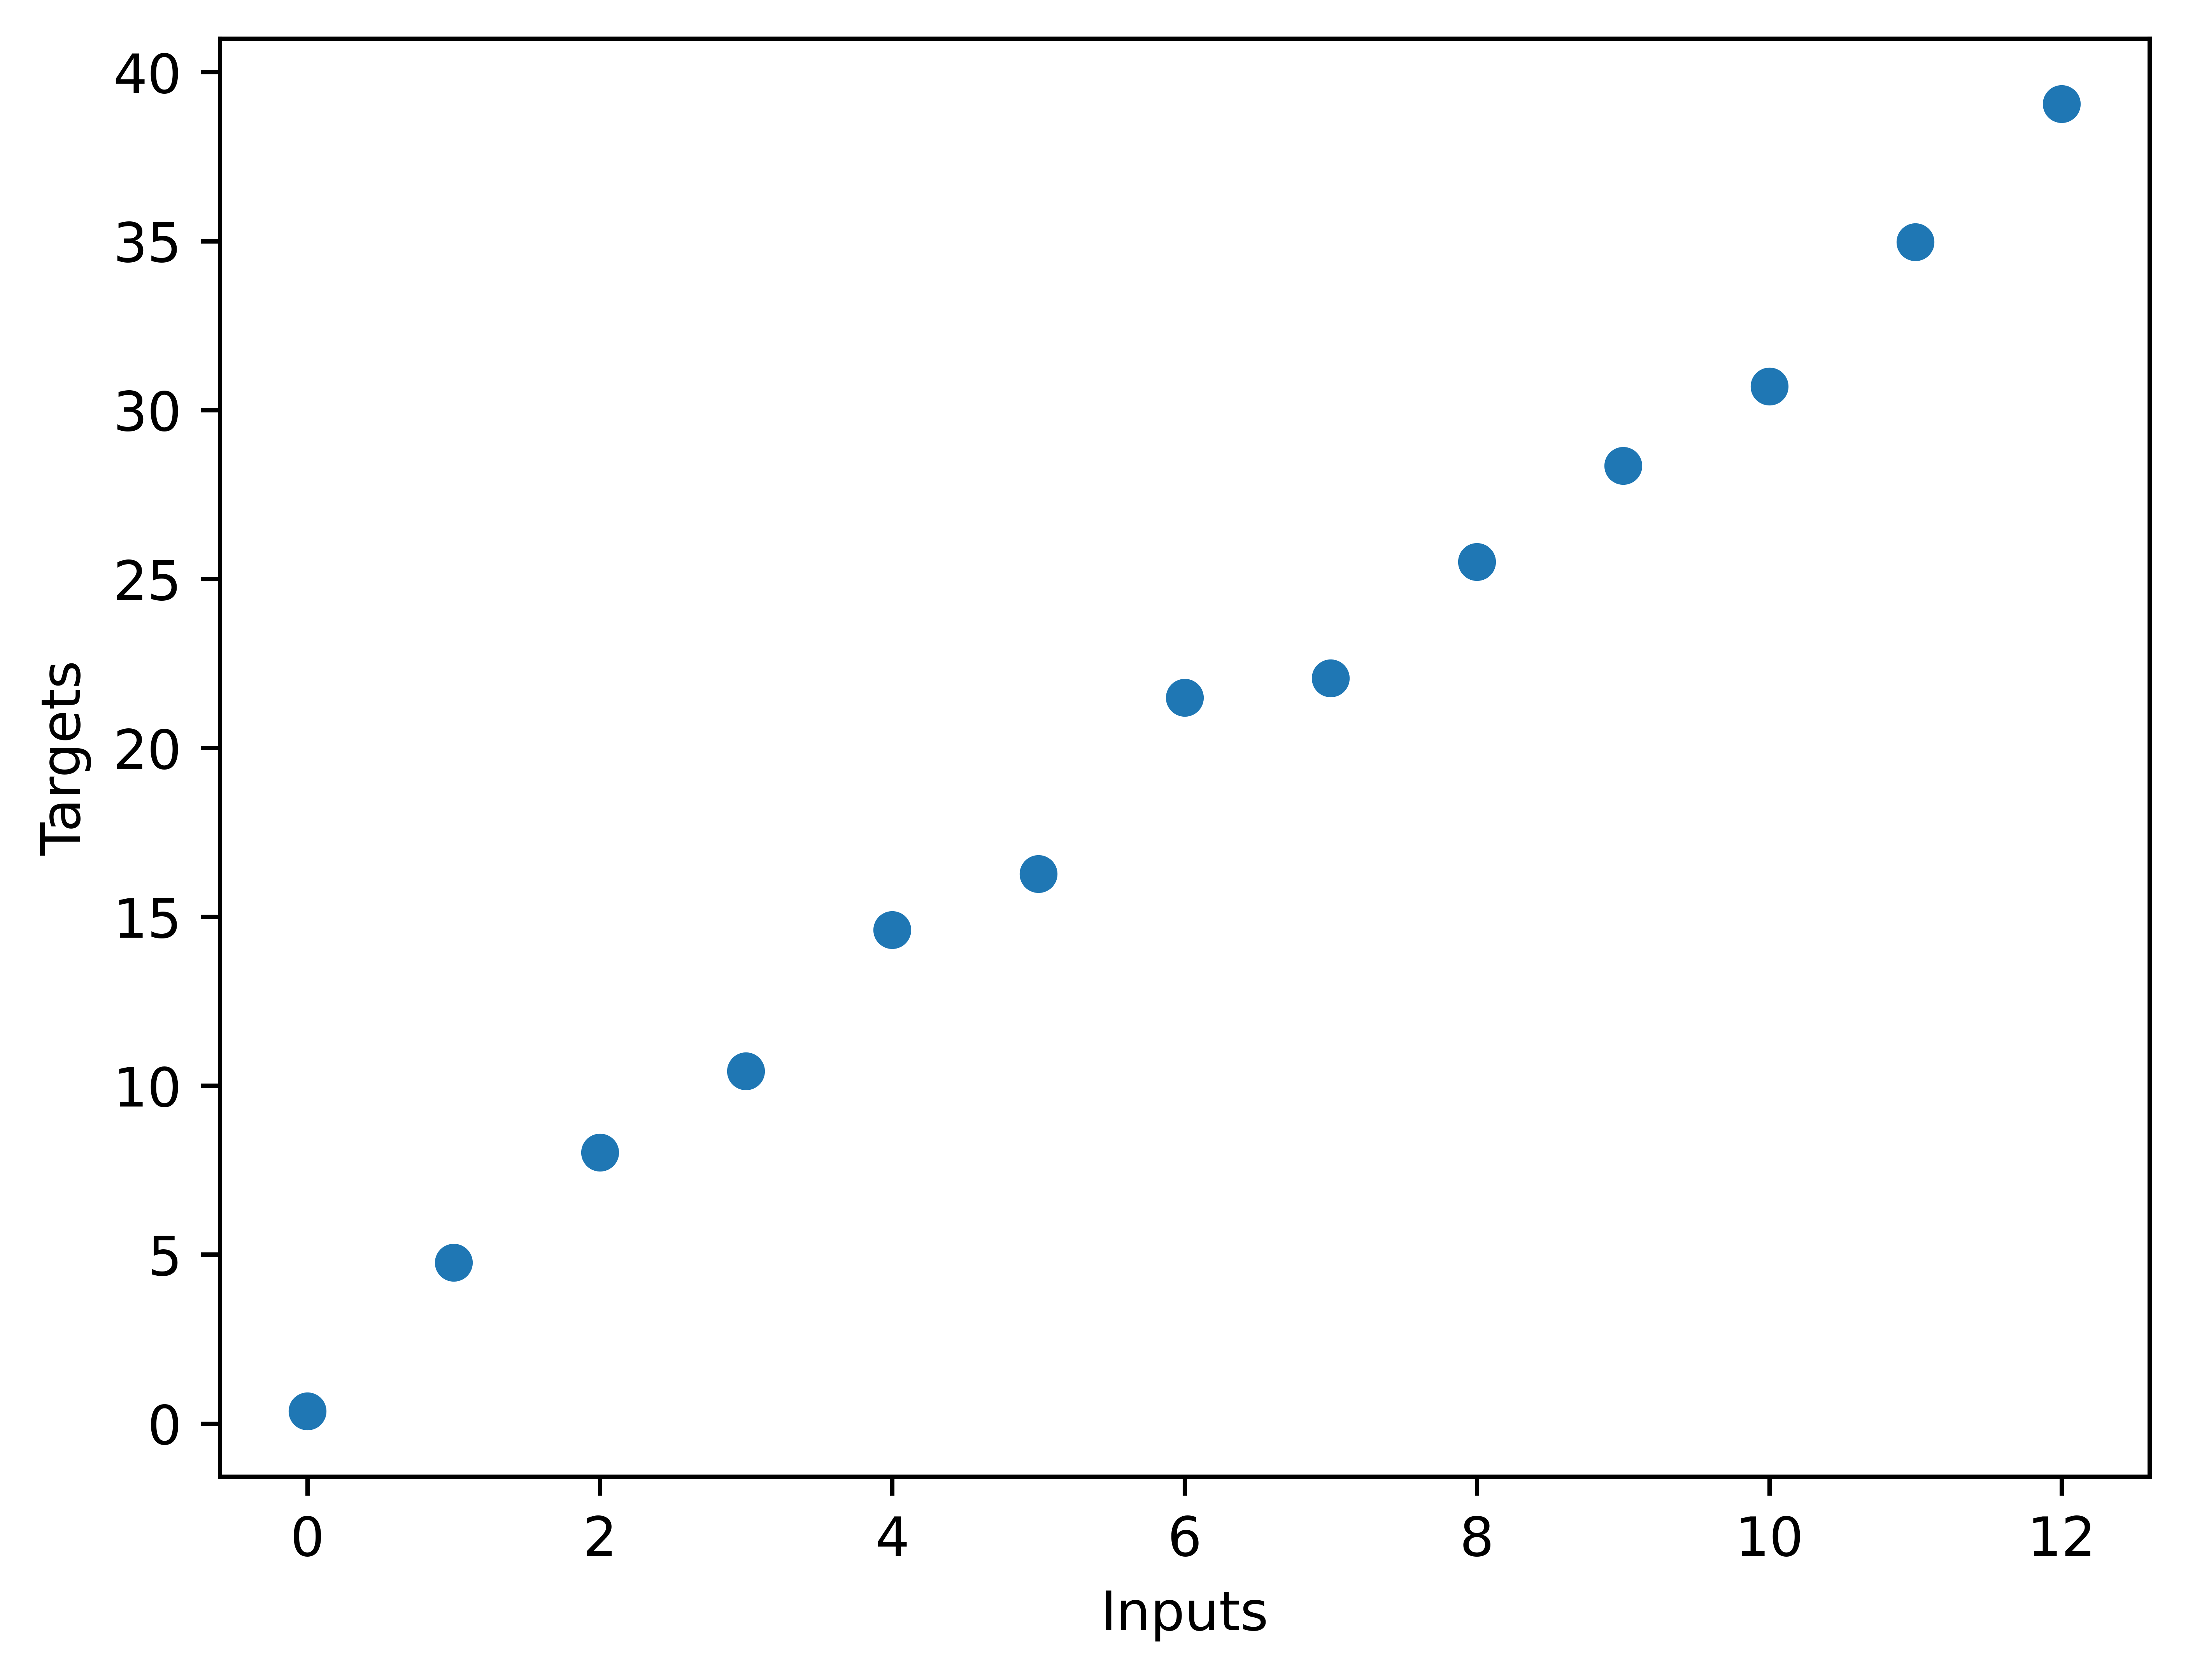
\includegraphics[scale=0.38]{pics/lin_regression_data.png}
	\end{minipage}
	\begin{lstlisting}
	    data = np.arange(0, 13, dtype=np.float32)
        labels = data * 3 + 2 + np.random.normal(0, 1, size=data.shape)
        labels = labels.astype(np.float32)
	\end{lstlisting}
	
	\framebreak
	
	\begin{minipage}{0.4\textwidth}
	\begin{block}{Modell (low-level)}
	\begin{itemize}
		\item Modell-Parameter:
	\end{itemize}
	\begin{lstlisting}
	w = tf.Variable([0.5])
    b = tf.Variable([10.0])
	\end{lstlisting}
	\begin{itemize}
	 	\item Lineares Modell:
	 \end{itemize}
	\begin{lstlisting}
	def linear_model(inputs):
        return w * inputs + b
	\end{lstlisting}
	\end{block}
	\end{minipage}
	\begin{minipage}{0.58\textwidth}
	    \vspace*{5mm}
	    \centering
        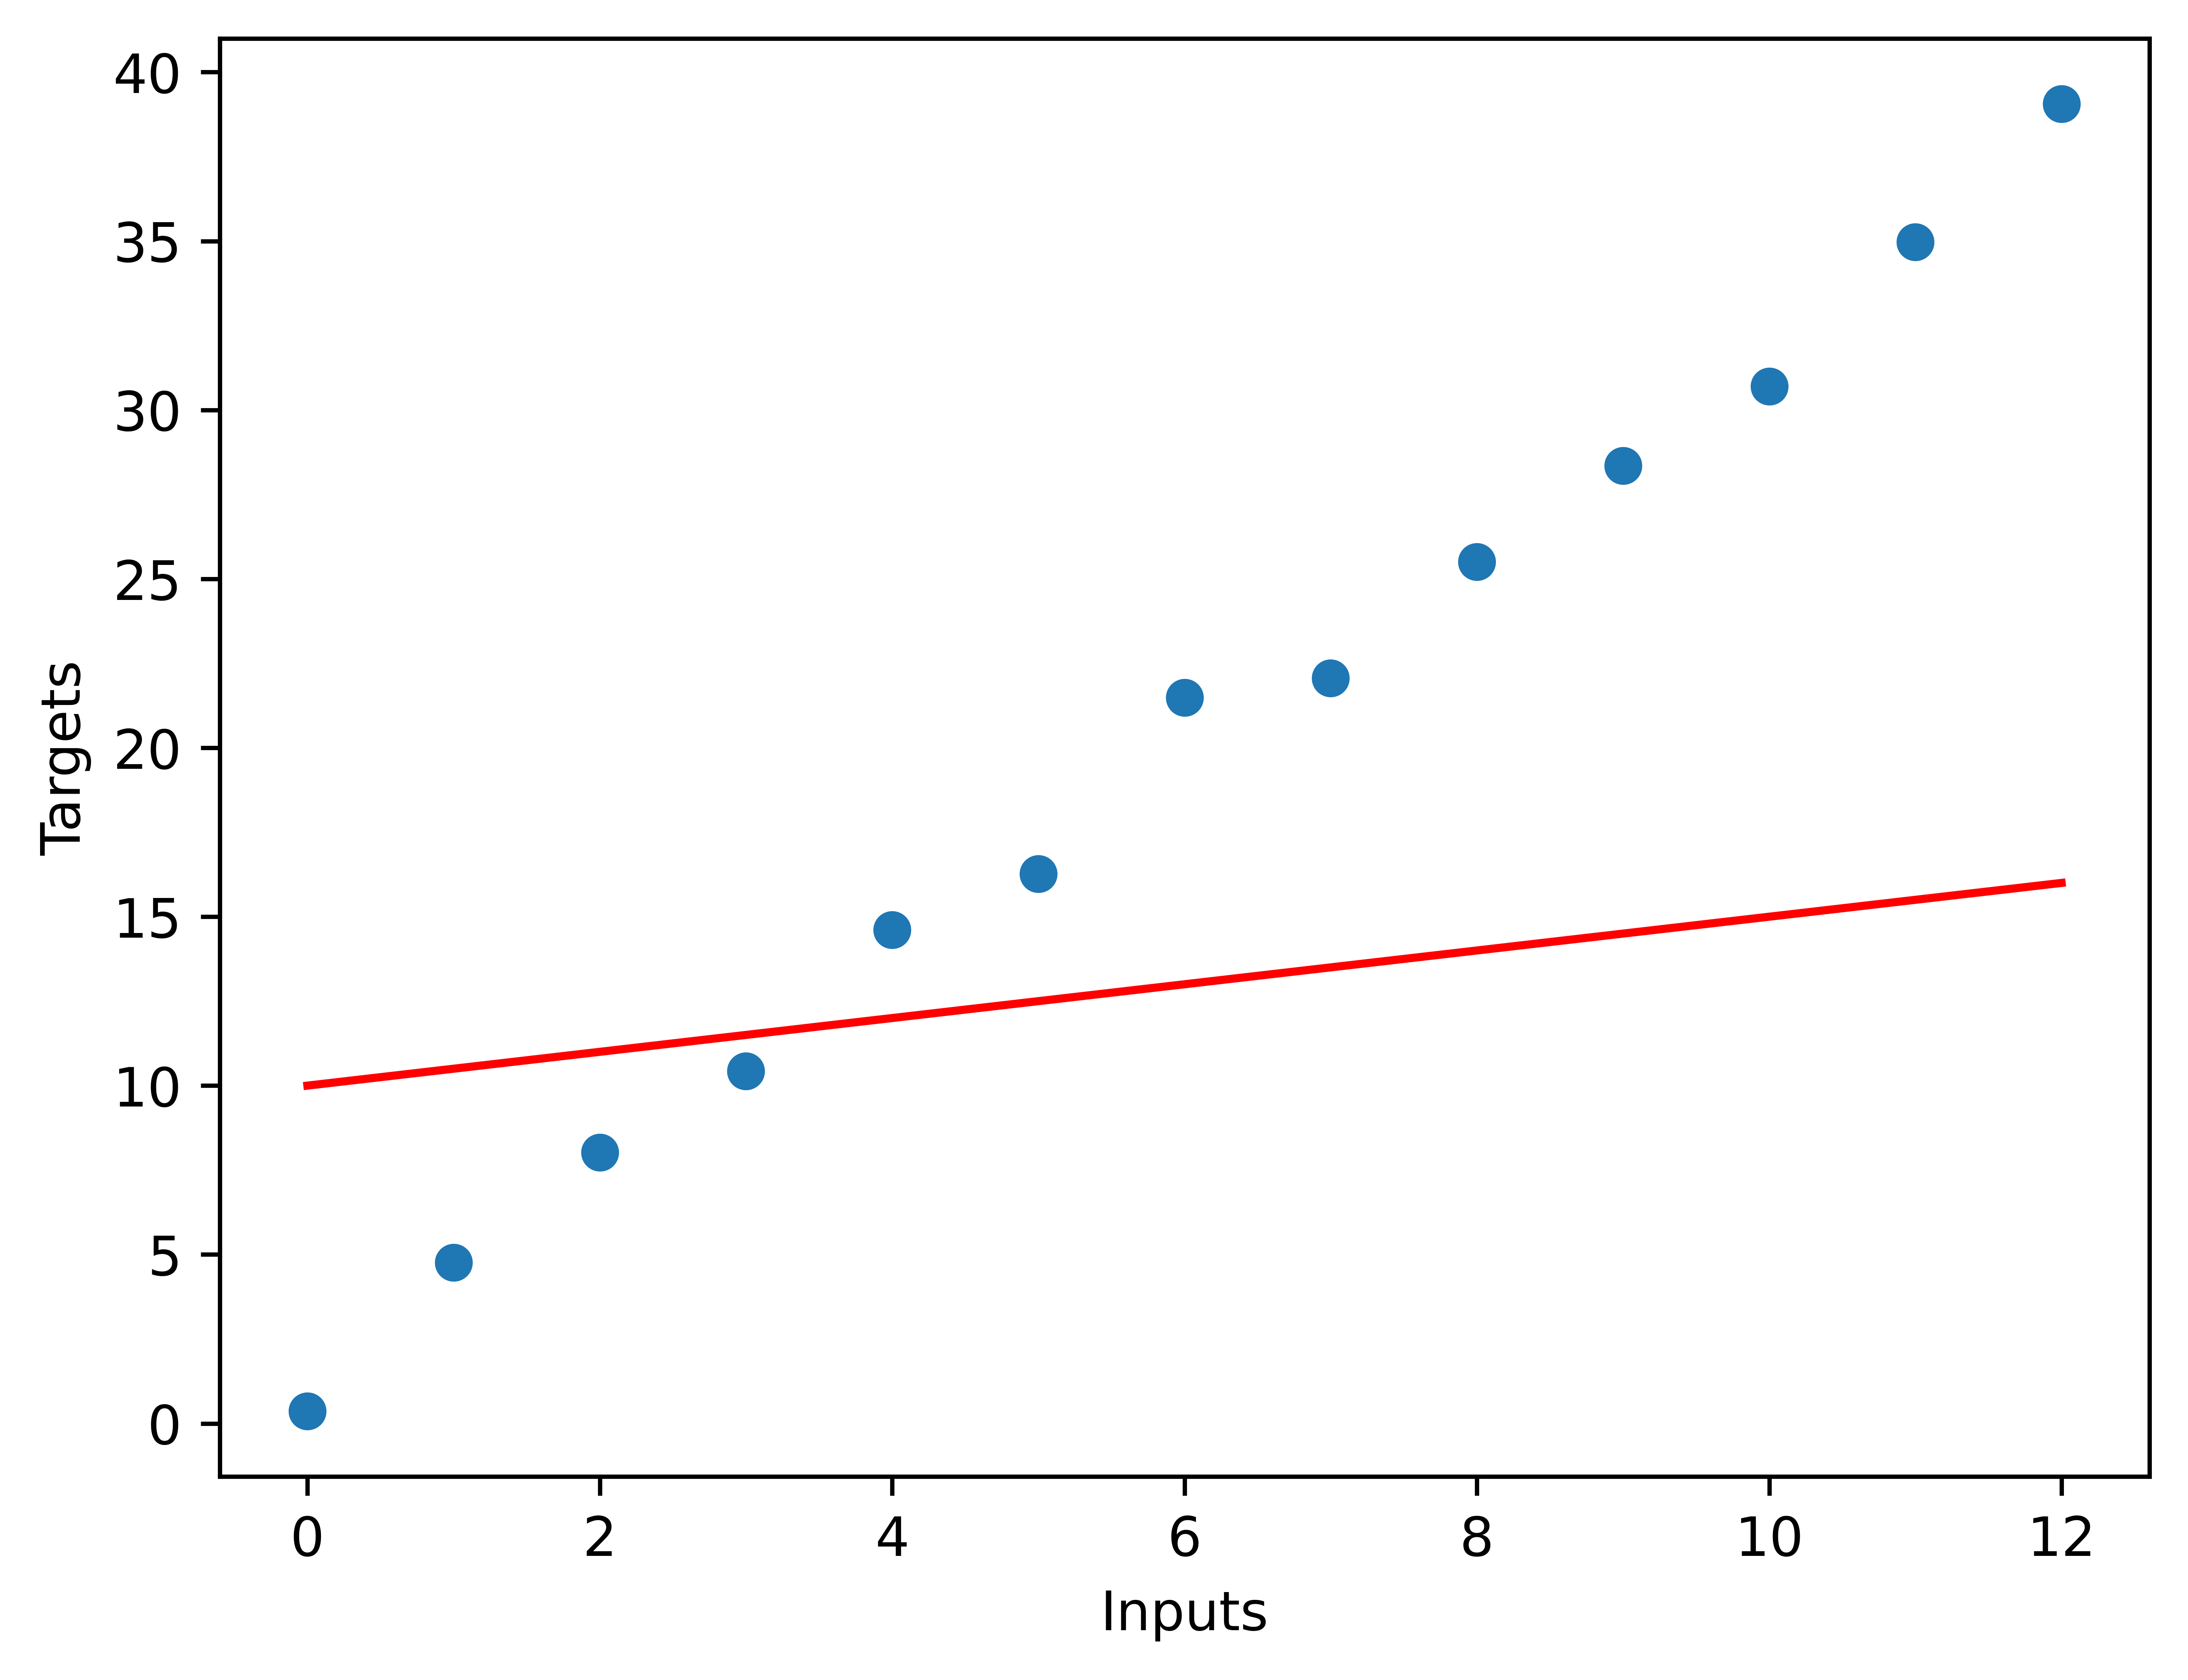
\includegraphics[scale=0.38]{pics/lin_regression_model_initial.png}
	\end{minipage}
	
	\framebreak
	
	\begin{block}{Modell-Performance}
	\begin{itemize}
		\item \textbf{Fehlerfunktion} (loss function) misst den Fehler zwischen den Vorhersagen des Modells und den gewünschten Ausgaben
		\item Standardzielfunktion für lineare Regression: Mittelwert der Fehlerquadrate: $\mathcal{L} = \frac{1}{n}\sum_{i=1}^n (y_i - f(x_i))^2$
	\end{itemize}
	\begin{lstlisting}
	    def loss_fn(inputs, targets):
            return tf.reduce_mean(tf.square(targets - inputs))
	\end{lstlisting}
	\begin{itemize}
	    \item Diverse Lossfunktionen im maschinellen Lernen \\$\rightarrow$ TensorFlow \tt{keras.losses} \\({\footnotesize\url{tensorflow.org/api_docs/python/tf/keras/losses}})
	\end{itemize}
	\begin{lstlisting}
	    tf.keras.losses.mean_squared_error(targets, linear_model(inputs))
	\end{lstlisting}
	\end{block}
	
	\framebreak
	
	\begin{block}{Modell-Optimierung}
	\begin{itemize}
		\item Diverse Optimierungsverfahren im maschinellen Lernen \\$\rightarrow$ TensorFlow \tt{keras.optimizers} \\({\footnotesize\url{tensorflow.org/api_docs/python/tf/keras/optimizers}})
		\item Optimierer versuchen die Lossfunktion zu minimieren, indem die zugrundeliegenden Modellvariablen angepasst werden
		\item Grundidee: \textbf{Gradientenabstieg} zum Finden lokaler/globaler Minima\\$\rightarrow$ Variablen werden in Richtung des negativen Gradienten der Fehlerfunktion verschoben (hier: $-\frac{\partial\mathcal{L}}{\partial w}$ bzw. $-\frac{\partial\mathcal{L}}{\partial b}$).
	\end{itemize}
	\begin{lstlisting}
	    optimizer = tf.keras.optimizers.SGD(learning_rate=0.01)
	\end{lstlisting}
	\end{block}
	
	\framebreak
	
	\begin{block}{Gradientenabstieg}
	    \begin{itemize}
	        \item Gradientenabstieg für Funktion $J\colon\mathbb{R}^n \rightarrow \mathbb{R}$
			\begin{align*}
			\mathbf{w}^{(i+1)} = \mathbf{w}^{(i)} - \alpha\nabla f(\mathbf{w}^{(i)})
			\end{align*}
	    \end{itemize}
	    \centering
		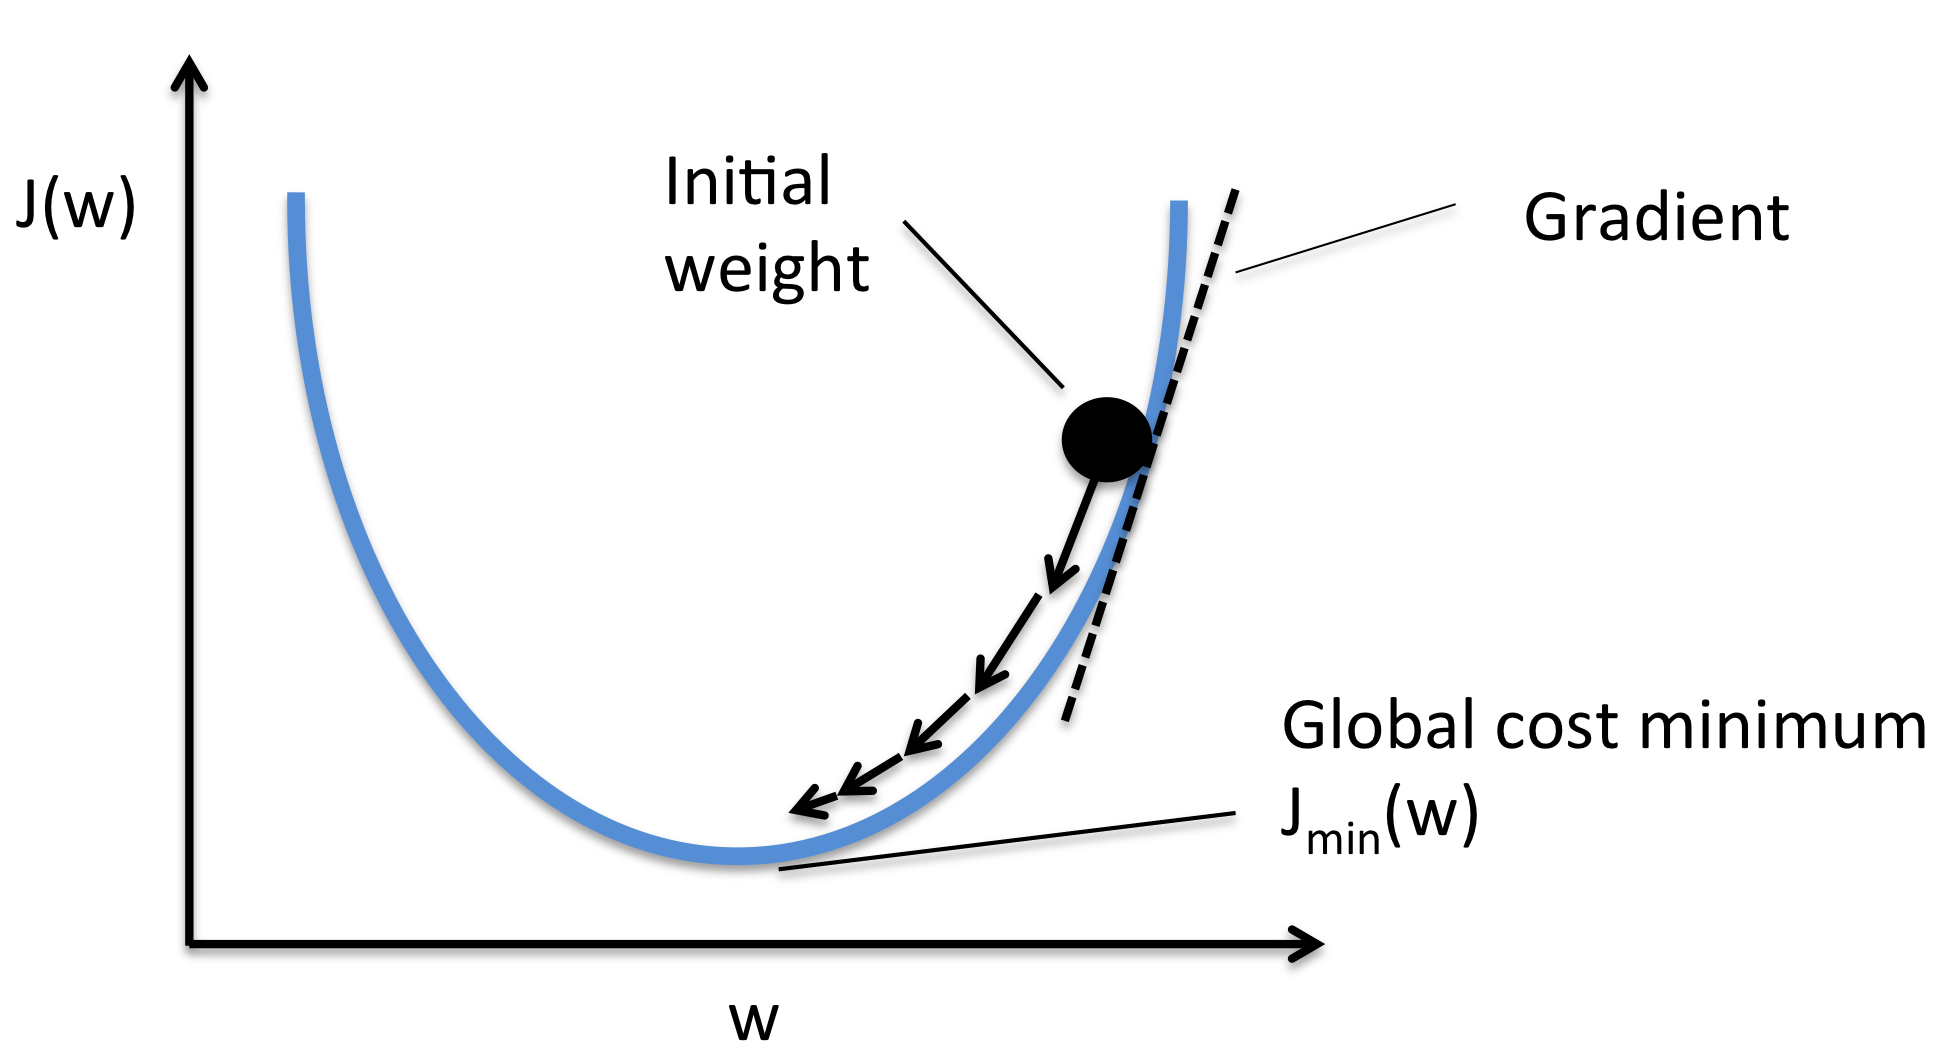
\includegraphics[scale=0.09]{pics/gradient_descent}
		{\tiny\url{rasbt.github.io/mlxtend/user_guide/general_concepts/gradient-optimization}}
	\end{block}
		
	\framebreak
	
	\begin{block}{Berechnung der Gradienten}
	    \begin{itemize}
	        \item TensorFlow unterstützt automatische Differentiation
	        \item \tt{tf.GradientTape()} erzeugt eine Umgebung in der TensorFlow Operationen zur automatischen Differentiation aufgezeichnet werden
	        \item \tt{tape.gradient(target, sources)} berechnet die Gradienten der \textit{target} Tensoren bzgl. der \textit{sources} Variablen
	    \end{itemize}
	    \begin{lstlisting}
        @tf.function
        def gradients(inputs, targets):
            with tf.GradientTape() as tape:
                outputs = linear_model(inputs)
                loss = loss_fn(outputs, targets)
                grads = tape.gradient(loss, [w, b])
            return loss, grads
	    \end{lstlisting}
	\end{block}
	
	\framebreak
	
	\begin{block}{Modell-Training}
	    \begin{itemize}
	        \item Mehrfach über den Datensatz iterieren (\textit{Epochen})
	        \item Gradienten berechnen
	        \item Optimierungsschritt durchführen \\$\rightarrow$ \tt{optimizer.apply\_gradients(grads\_and\_vars)}, wobei \textit{grads\_and\_vars} eine Liste von Tupeln \textit{(gradient, variable)} ist
	    \end{itemize}
	    \begin{lstlisting}
        num_epochs = 300
        for epoch in range(num_epochs):
            loss, grads = gradients(data, labels)
            optimizer.apply_gradients(zip(grads, [w, b]))
	    \end{lstlisting}
	\end{block}
	
	\framebreak
	
	\begin{itemize}
	    \item Modell-Evaluation
	\end{itemize}
	\begin{minipage}{0.49\textwidth}
	    \centering
	    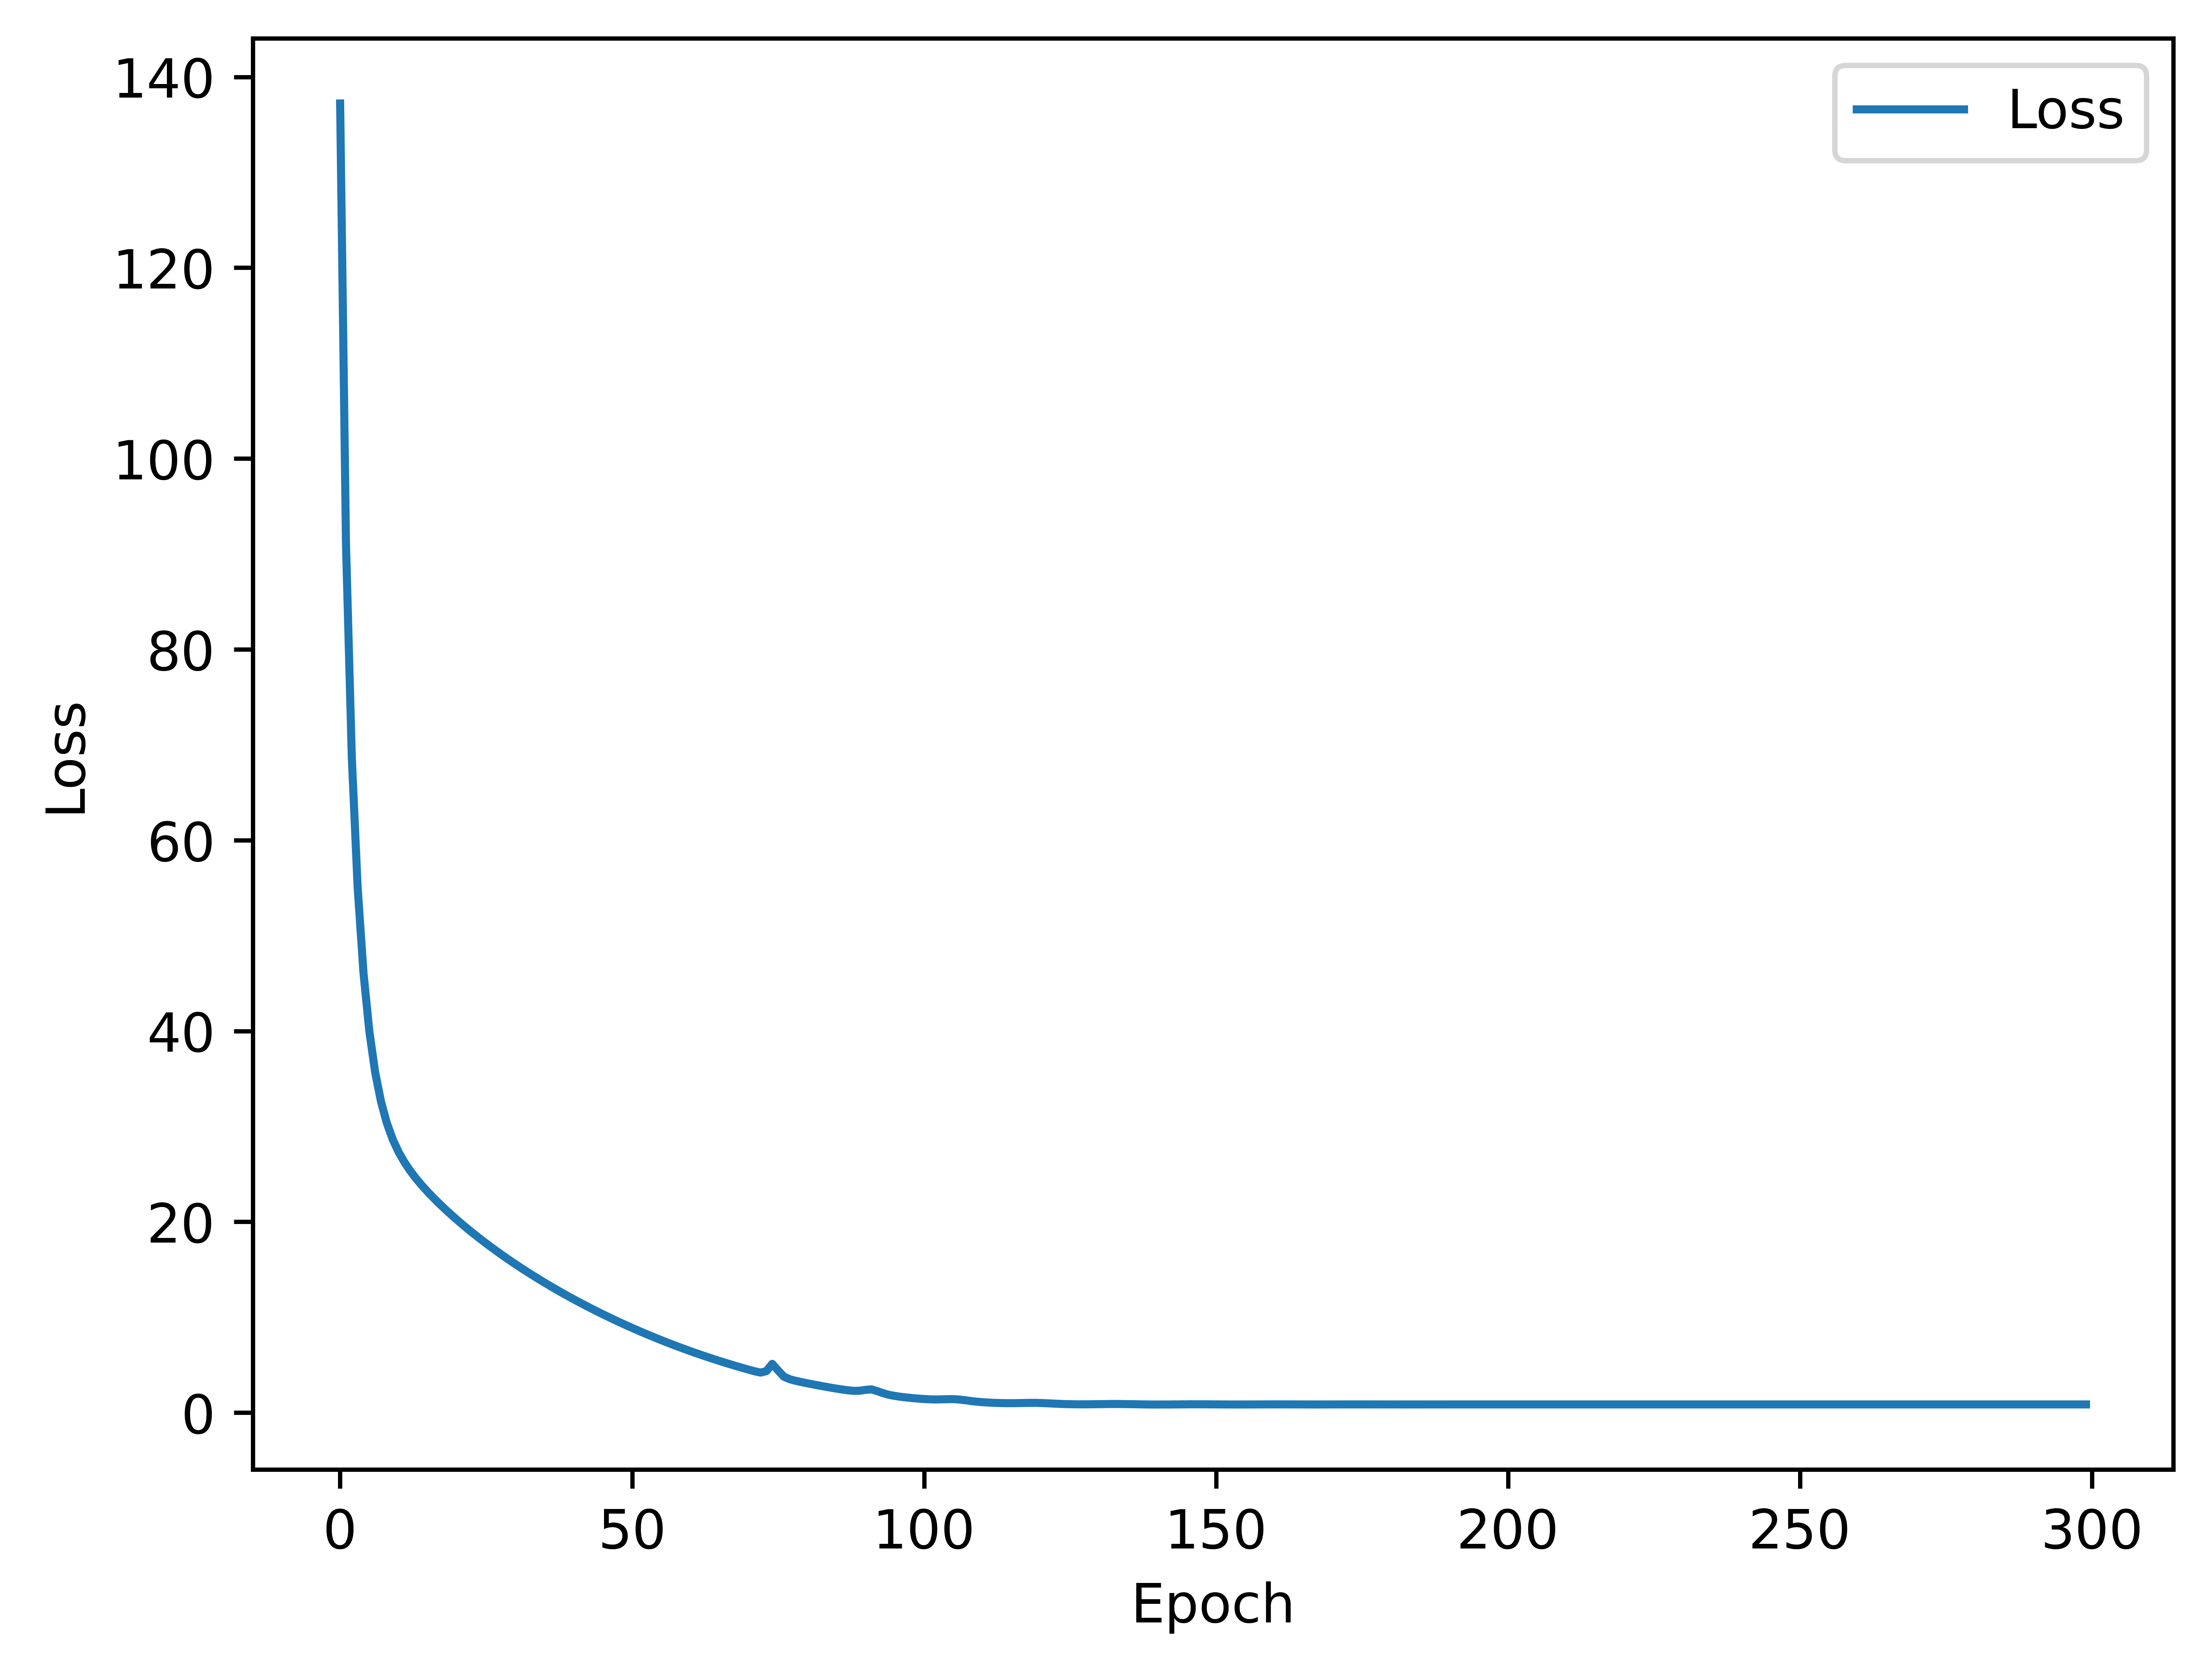
\includegraphics[scale=0.35]{pics/lin_regression_loss_curve.png}
	\end{minipage}
	\begin{minipage}{0.49\textwidth}
	    \centering
	    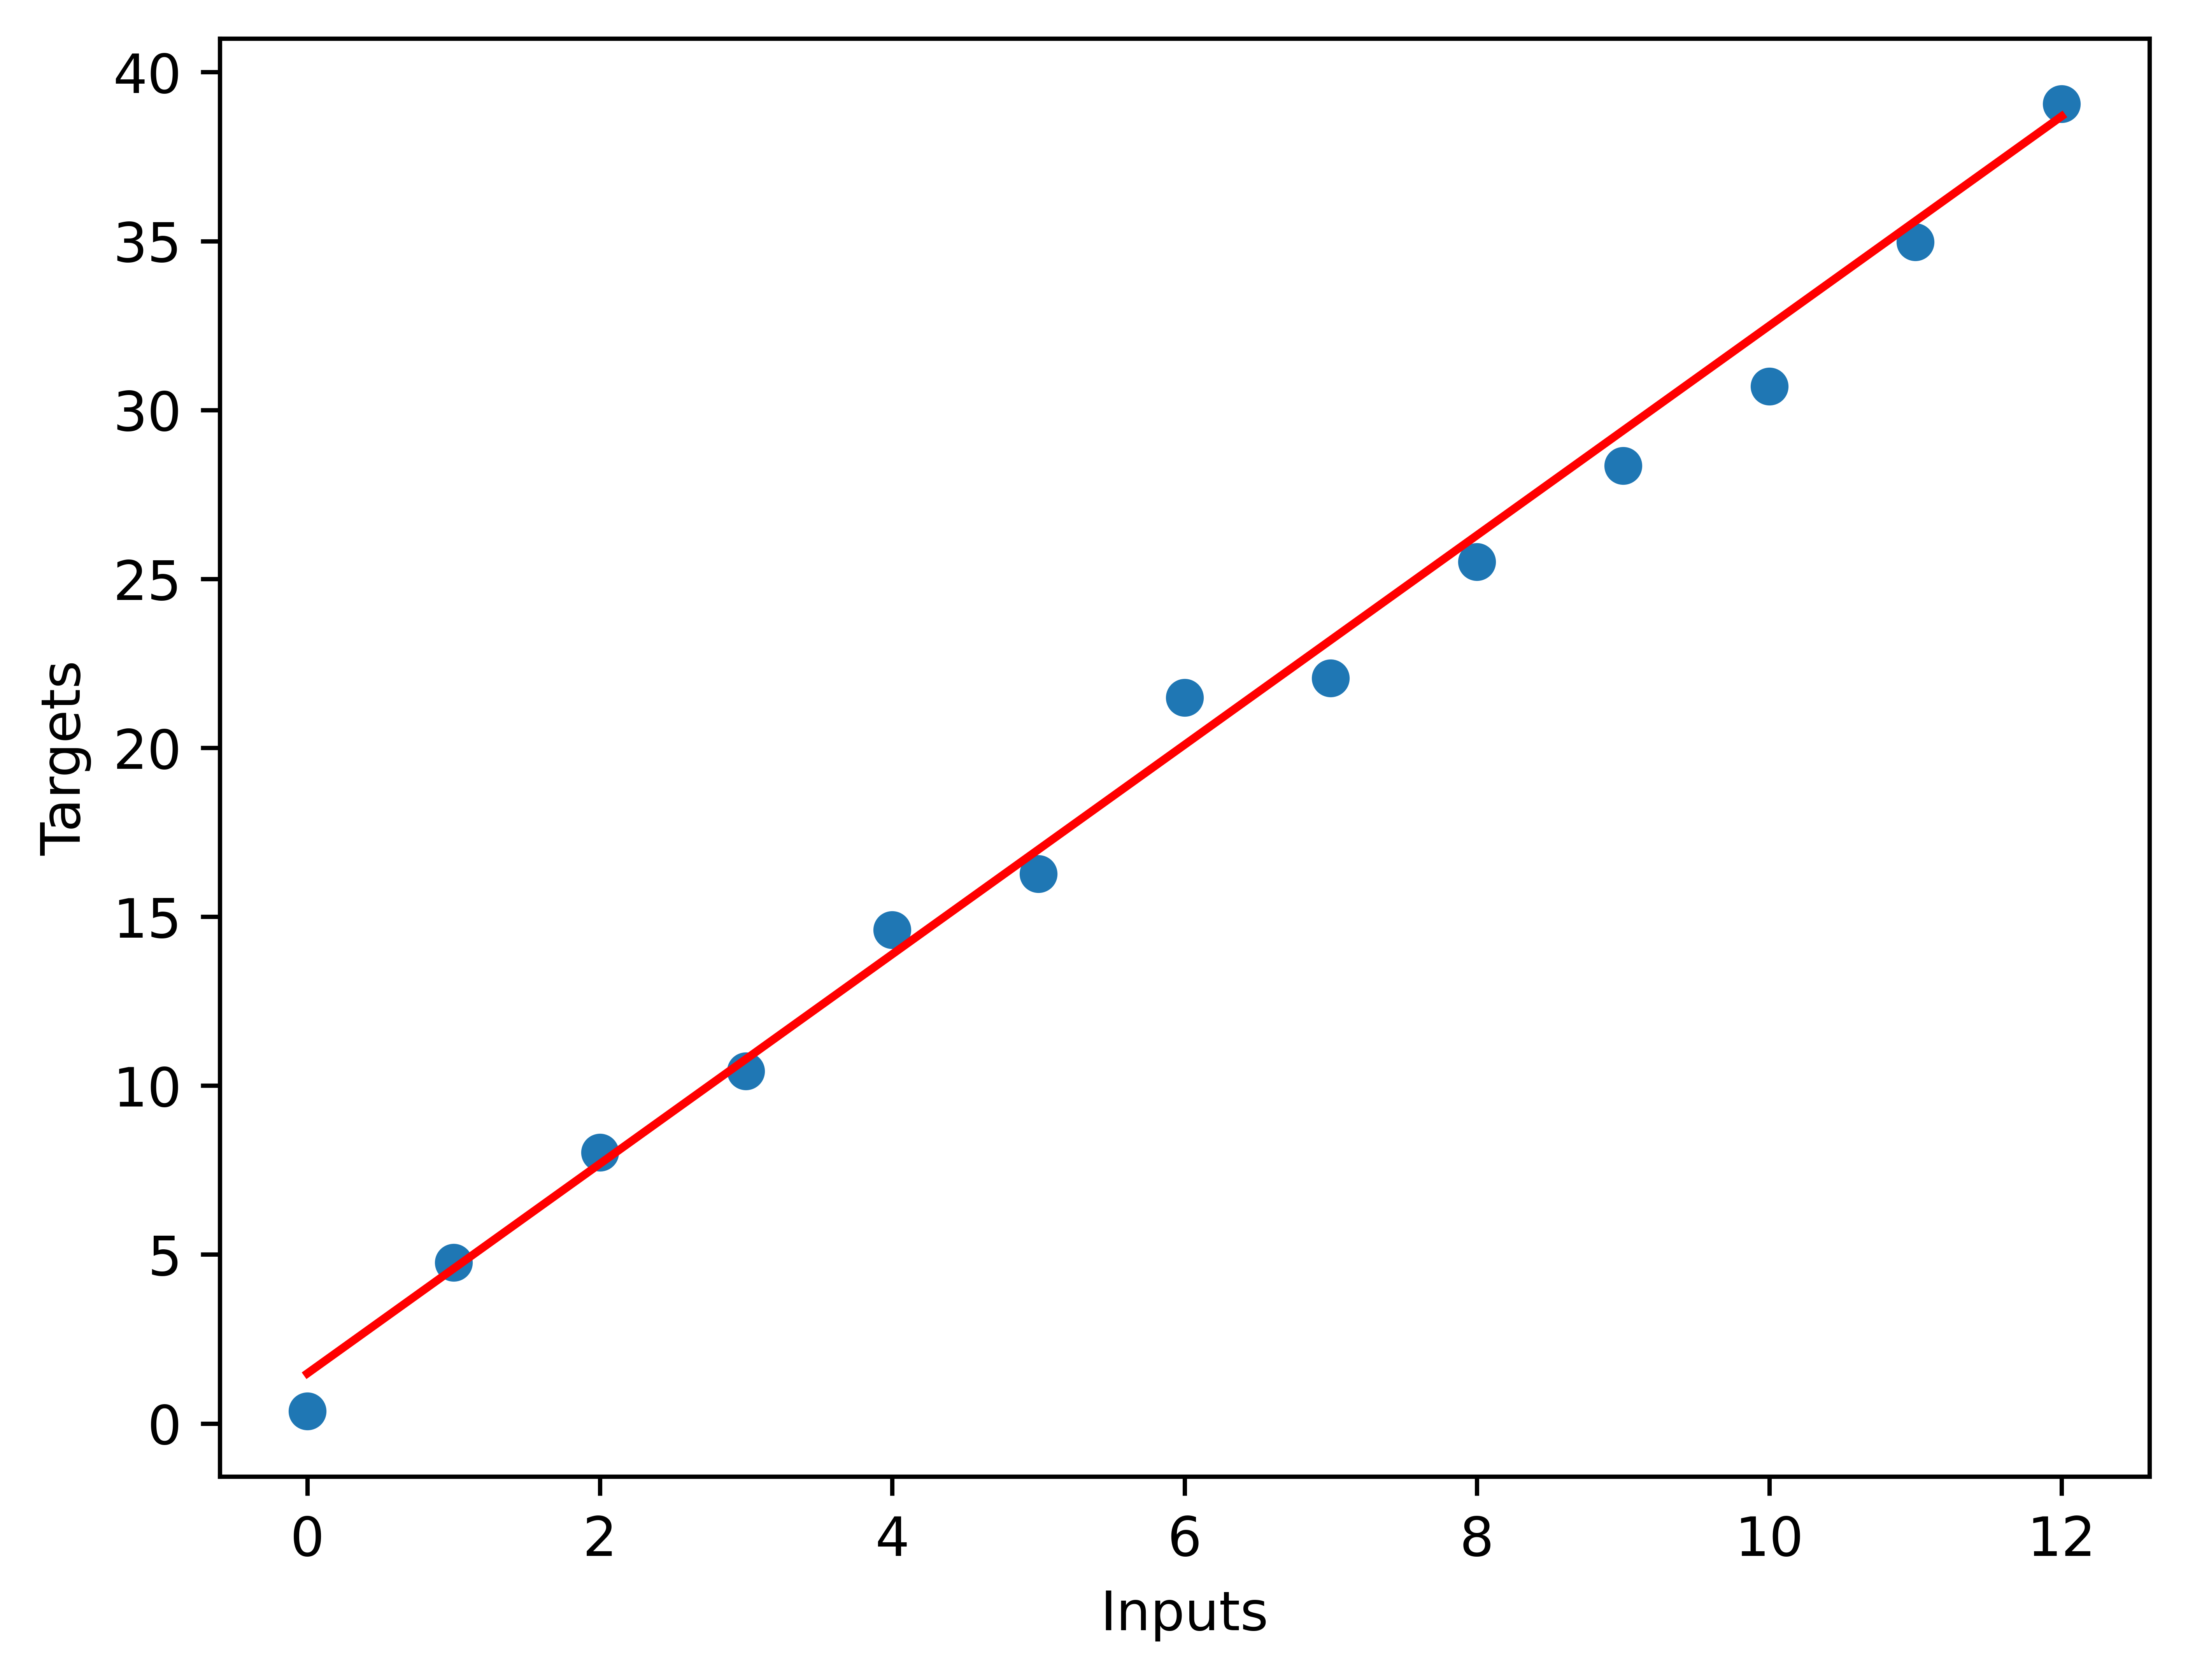
\includegraphics[scale=0.35]{pics/lin_regression_model_trained.png}
	\end{minipage}
	\begin{itemize}
	    \item Trainierte Paramter: $w=[3.1010873]$, $b=[1.4811424]$
	\end{itemize}
	
	\framebreak
	
	\begin{block}{\tt{tf.keras}}
	    \begin{itemize}
	        \item Erlaubt es komplexere Modelle aus vordefinierten Schichten (\tt{keras.layers}) zusammenzubauen
	        \begin{itemize}
	            \item \textit{Sequential} API (\tt{keras.models.Sequential})
	            \item \textit{Functional} API (\tt{keras.Model(inputs, outputs)})
	            \item \textit{Subclassing} API (eigene \tt{layers}, \tt{Models})
	            \item[$\rightarrow$] Bequemlichkeit vs. Flexibilität
	        \end{itemize}
	        \item Ein \tt{layer} kapselt seine Variablen (Gewichte, weights) und eine Input-Output-Transformation\\ ({\footnotesize\url{tensorflow.org/api_docs/python/tf/keras/layers}})
	        \item \tt{model.fit} übernimmt den gesamten Trainingsprozess eines \tt{keras} Modells und liefert eine \tt{history} über den Verlauf des Trainings
	    \end{itemize}
	\end{block}
	
	\framebreak
	
	\begin{block}{Sequential Modell}
	    \begin{itemize}
	        \item \tt{keras.model.Sequential} erhält eine Liste von \tt{keras.layers}, welche sequentiell ausgeführt werden
	        \item \tt{model.compile} erhält einen Optimierer, sowie eine Loss- und Metrikfunktion ({\footnotesize\url{tensorflow.org/api_docs/python/tf/keras/metrics}})
	    \end{itemize}
	    \begin{lstlisting}
def sequential_model(learning_rate):
    model = keras.models.Sequential(
                [keras.layers.Input(shape=(1,)),  # shape of a single input
                keras.layers.Dense(units=1)]) # fully-connected layer
    model.compile(optimizer=keras.optimizers.RMSprop(learning_rate=learning_rate),
                 loss=keras.losses.mean_squared_error,
                 metrics=[keras.metrics.mean_squared_error])
    return model
	    \end{lstlisting}
	\end{block}
	
	\framebreak
	
	\begin{block}{Modell-Training}
	    \begin{itemize}
	        \item \tt{model.fit} erhält
	        \begin{itemize}
	            \item die Eingabedaten und zugehörigen Targets
	            \item die \textit{batch\_size} (Größe der Blöcke/Batches in der die Daten verarbeitet werden)
	            \item die Anzahl der Epochen zum Trainieren
	        \end{itemize}
	        \item und liefert eine \tt{history} mit Informationen über die Epochen, den Loss und die Metrik
	    \end{itemize}
	    \begin{lstlisting}
        history = model.fit(x=inputs,
                       y=targets,
                       batch_size=batch_size,
                       epochs=epochs)
        epochs = history.epochs
        losses = history.history['loss']
        errors = history.history['mean_squared_error']
	    \end{lstlisting}
	\end{block}
\end{frame}

\begin{frame}[fragile]{Sonstiges}
    \begin{itemize}
        \item Modellausgaben erzeugen mit \tt{model.predict}
        \item In \tt{keras} aufbereitete Datensätze:
        \begin{itemize}
            \item \tt{keras.datasets.mnist.load\_data()}
            \item[$\rightarrow$] Multi-Klassifizierungsproblem (Ziffern 0-9)
            \item \tt{keras.datasets.fashion\_mnist.load\_data()}
            \item[$\rightarrow$] Multi-Klassifizierungsproblem (Kleidungsstücke)
            \item weitere siehe {\footnotesize\url{https://keras.io/api/datasets/}}
        \end{itemize}
    \end{itemize}
    
\end{frame}


%%%%%%%%%%%%%%%%%%%%%%%%%%%%%%%%%%%%%%%%%%%%%%%%%%%%%%%%%%%%%%%%%%%%%%%%%%%%%%%%%%%%%%%%%%%%%%%
%%%%%%%%%%%%%%%%%%%%%%%%%%%%%%%%%%%%%%%%%%%%%%%%%%%%%%%%%%%%%%%%%%%%%%%%%%%%%%%%%%%%%%%%%%%%%%%
%%%%%%%%%%%%%%%%%%%%%%%%%%%%%%%%%%%%%%%%%%%%%%%%%%%%%%%%%%%%%%%%%%%%%%%%%%%%%%%%%%%%%%%%%%%%%%%
\iffalse
\section{OLD}
%%%%%%%%%%%%%%%%%%%%%%%%
\section{MNIST Tutorial}
%%%%%%%%%%%%%%%%%%%%%%%%
\begin{frame}[fragile, allowframebreaks]{MNIST Tutorial}
	\begin{block}{Überblick}
		\begin{itemize}
			\item Kennenlernen des \textit{MNIST}-Datensatzes
			\item Softmax Regression (Multinomiale Logistische Regression)
			\item Erstellen ein Modell $f$, das auf Basis der Pixel im Bild eine Zuordnung zu einer Ziffer vornehmen kann 
			(Inference-Phase):
				\begin{align*}
					f\colon \mathbb{R}^{28\times 28} &\rightarrow \{0,1,2,3,4,5,6,7,8,9\} \text{\quad bzw.} \\
					f\colon \mathbb{R}^{784} &\rightarrow \{0,1,2,3,4,5,6,7,8,9\}
				\end{align*}
			\item Trainieren das Modell mit Tausenden Beispielen (Trainings-Phase)
			\item Prüfen wie gut das Modell arbeitet (Test-Phase)
		\end{itemize}
	\end{block}
	
	\framebreak

	\begin{block}{MNIST Datensatz}
		\begin{itemize}
			\item MNIST = \textbf{M}odified \textbf{N}ational \textbf{I}nstitute of \textbf{S}tandards and
			\textbf{T}echnology
			\item "Hello World" des Maschinellen Lernens
			\item Datenbank handgeschriebener Ziffern
			\item Bilder der Grösse $28 \times 28$ Pixel
			\item Klassifikationsproblem: Bild $\rightarrow$ Ziffer
		\end{itemize}			
		\begin{figure}[c!]
			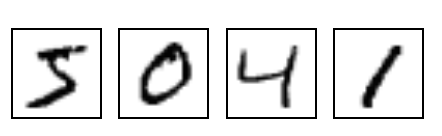
\includegraphics[scale=0.3]{pics/mnist_digits}
			\caption{Beispiele für MNIST-Ziffern.}
		\end{figure}				
	\end{block}	 
	
	\framebreak
	
	\begin{block}{Daten importieren}
		\begin{itemize}
			\item Unterteilung in Trainings-, Validierungs- und Testdaten
			\item Eingebaute Funktion zum Laden der Bilder, die in \verb+save_dir+ gespeichert werden:
			\begin{lstlisting}
	from tensorflow.examples.tutorials.mnist import input_data
	mnist = input_data.read_data_sets(save_dir, one_hot=True)
			\end{lstlisting}
			\item $55.000$ Trainingsdaten (\verb+mnist.train+)\\
			      $10.000$ Testdaten (\verb+mnist.test+)\\
			       $5.000$ Validierungsdaten (\verb+mnist.validation+)
		\end{itemize}
		
	\end{block}
	
	\framebreak
	
	\begin{block}{Interpretation der Daten I}
		\footnotesize
		\begin{itemize}
			\item Daten bestehen aus dem $28\times 28$ Bild $\mathbf{x}$ einer handgeschrieben Ziffer und dem zugehörigen
			Label $y$ aus $\{0, \dots, 9\}$
			\item Zugriff auf die Bilder und Label durch \tt{mnist.train.images} bzw. \tt{mnist.train.labels}
			\item Jedes Bild kann als Matrix interpretiert werden
		\end{itemize}
		\begin{figure}[c]
			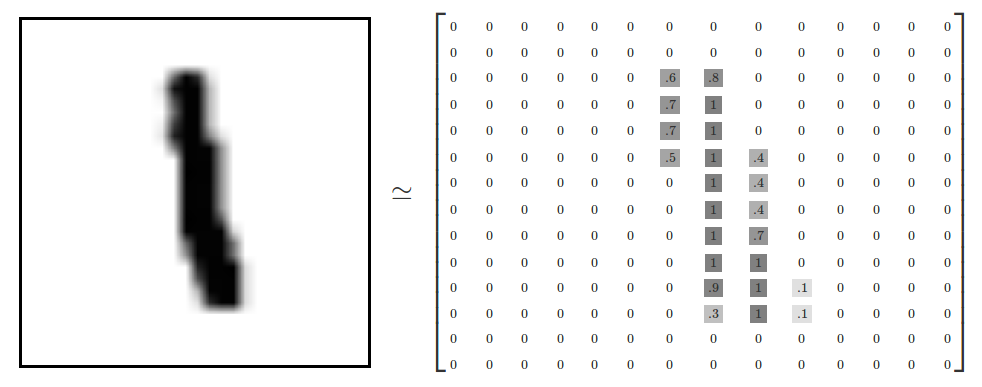
\includegraphics[scale=0.12]{pics/mnist_matrix}
			\caption{Interpretation der MNIST-Bilder als Matrix.}
		\end{figure}
	\end{block}		
	
	\framebreak
	
	\begin{block}{Interpretation der Daten II}
	\footnotesize
		\begin{itemize}
			\item Umwandeln der Matrix in einen Vektor der Länge $28\times 28 = 784$
			\item Schreiben dabei die Zeilen der Matrix hintereinander
			\item Informationen der 2D Struktur der Bilder gehen verloren
			\item \tt{mnist.train.images} ist ein Tensor mit shape $[55000, 784]$
		\end{itemize}
		\begin{figure}[c]
		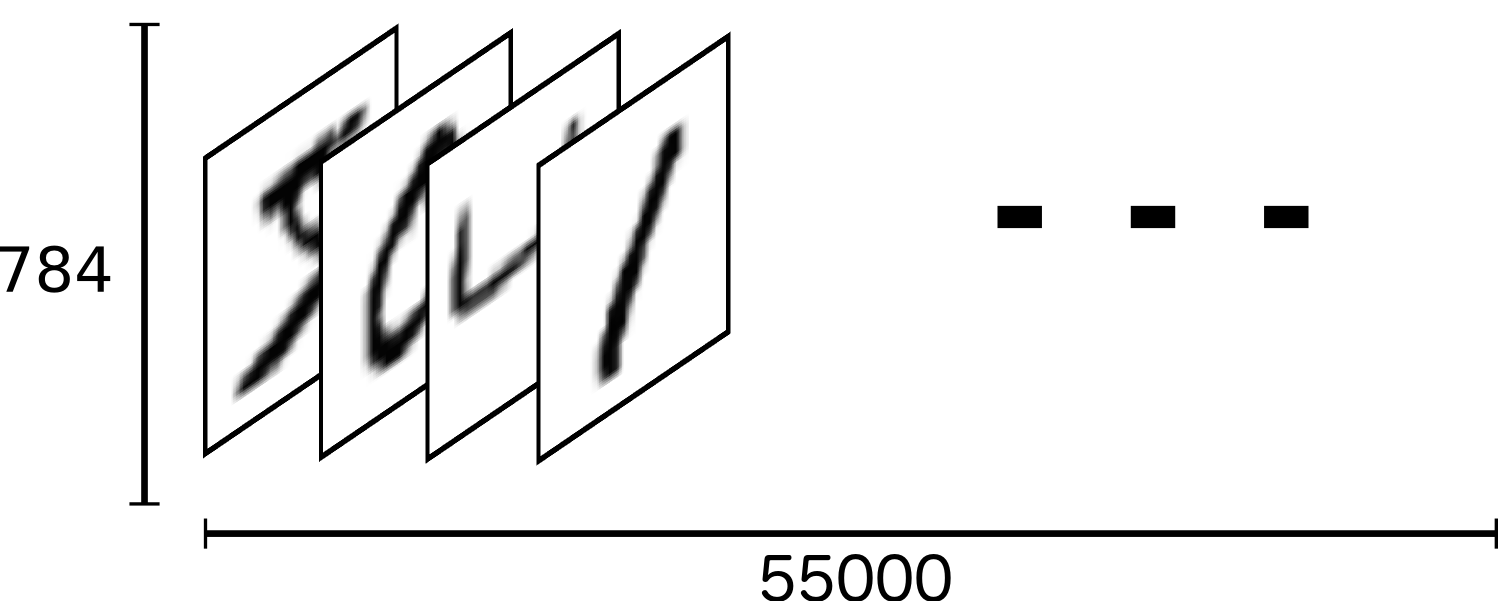
\includegraphics[scale=0.085]{pics/mnist_train_xs}
		\caption{$55.000$ Trainingsbilder als Vektoren der Länge $784$.}
		\end{figure}
	\end{block}
	
	\framebreak
	
	\begin{block}{Interpretation der Daten III}
		\footnotesize
		\begin{itemize}
			\item Fassen jedes Label $y\in\{0,\dots,9\}$ als \textit{one-hot-Vektor} $\mathbf{y}$ auf:
			\begin{align*}
				\mathbf{y} \in \{0,1\}^{10} \text{ mit } \mathbf{y}_i = \begin{cases} 1, \text{ falls } y = i \\
				0, \text{ sonst} \end{cases}  
			\end{align*}
			\item \tt{mnist.train.labels} ist ein Tensor mit shape $[55000, 10]$
		\end{itemize}
		\begin{figure}[c]
			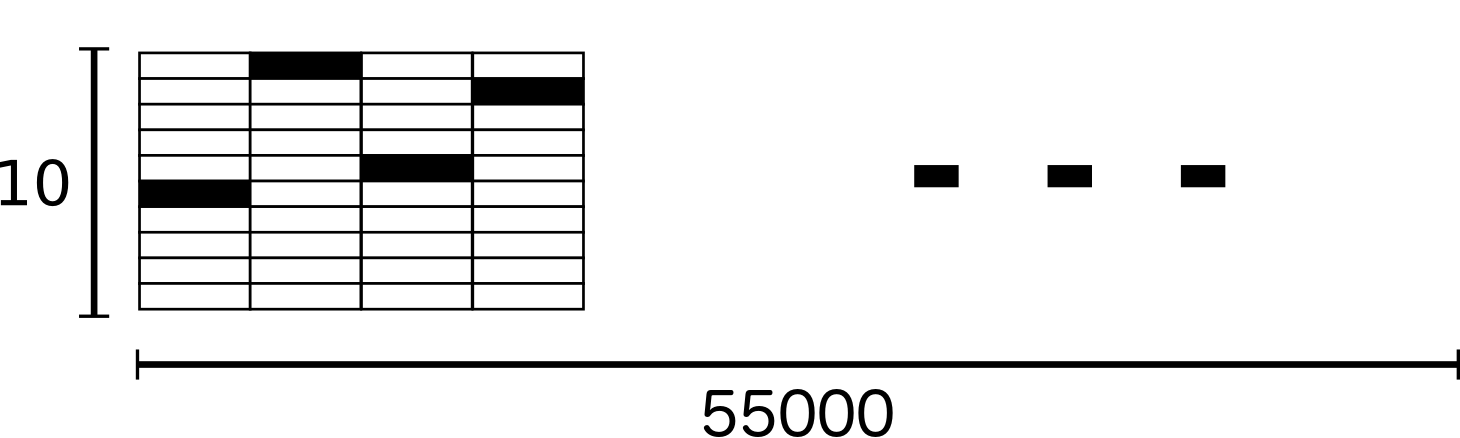
\includegraphics[scale=0.085]{pics/mnist_train_ys}
			\caption{$55000$ Trainingslabel als one-hot-Vektoren der Länge $10$.}
		\end{figure}					
	\end{block}
	
	\begin{block}{Softmax Regression I}
		\begin{itemize}
			\item Ziel: Für jedes Bild die Wahrscheinlichkeiten bestimmen, dass es sich um eine bestimmte Ziffer
			handelt $\rightarrow$ Softmax Regression
			\item Softmax liefert eine Liste von Werten zwischen $0$ und $1$ die sich zu $1$ aufsummieren
			\item Jede Ziffer erhält für ein bestimmtes Bild eine Gewichtung $\mathbf{z}$ die in eine
			Wahrscheinlichkeitsverteilung umgewandelt wird
			\begin{align*}
				&\mathbf{z} = W\mathbf{x} + \mathbf{b} \\
				&\mathbf{y} = softmax(\mathbf{z})\\
				&softmax(\mathbf{z})_i = \frac{\exp(z_i)}{\sum_j\exp(z_j)}
			\end{align*}
		\end{itemize}			
	\end{block}
	
	\framebreak
	
	\begin{block}{Softmax Regression II}
		Allgemeiner Aufbau
		\begin{figure}[c]
			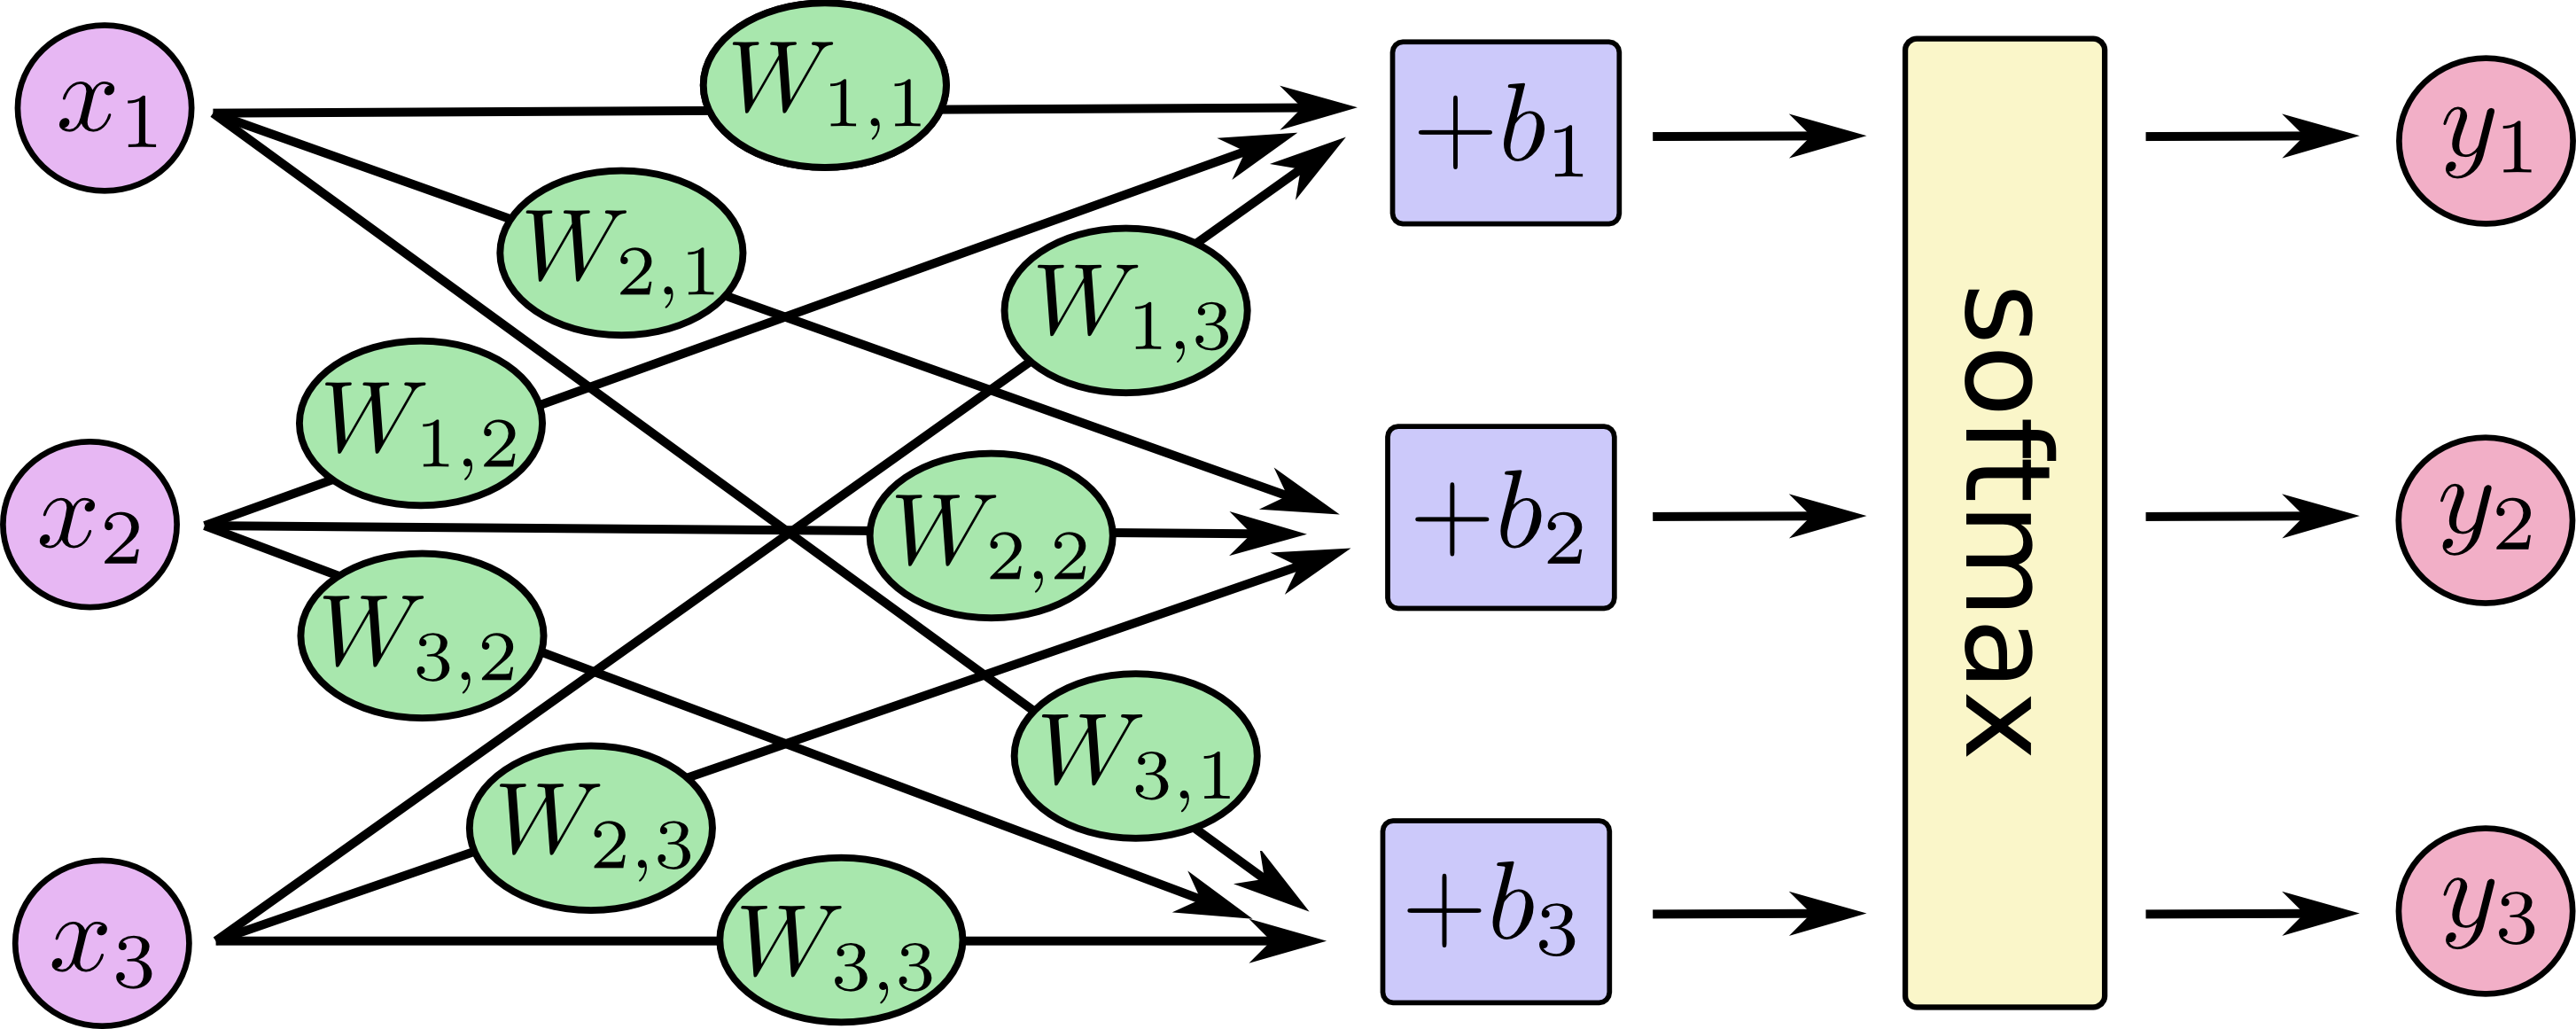
\includegraphics[scale=0.08]{pics/softmax_regression_scalargraph}
			\caption{Softmax Regression mit Eingaben $\mathbf{x}$ und Ausgaben $\mathbf{y}$.}
		\end{figure}
	\end{block}
	
	\framebreak
	
	\begin{block}{Softmax Regression III}
		Benutze Matrix-Vektor-Multiplikation anstatt die Werte einzeln zu berechnen
		\vspace{2pt}
		\begin{figure}[c]
			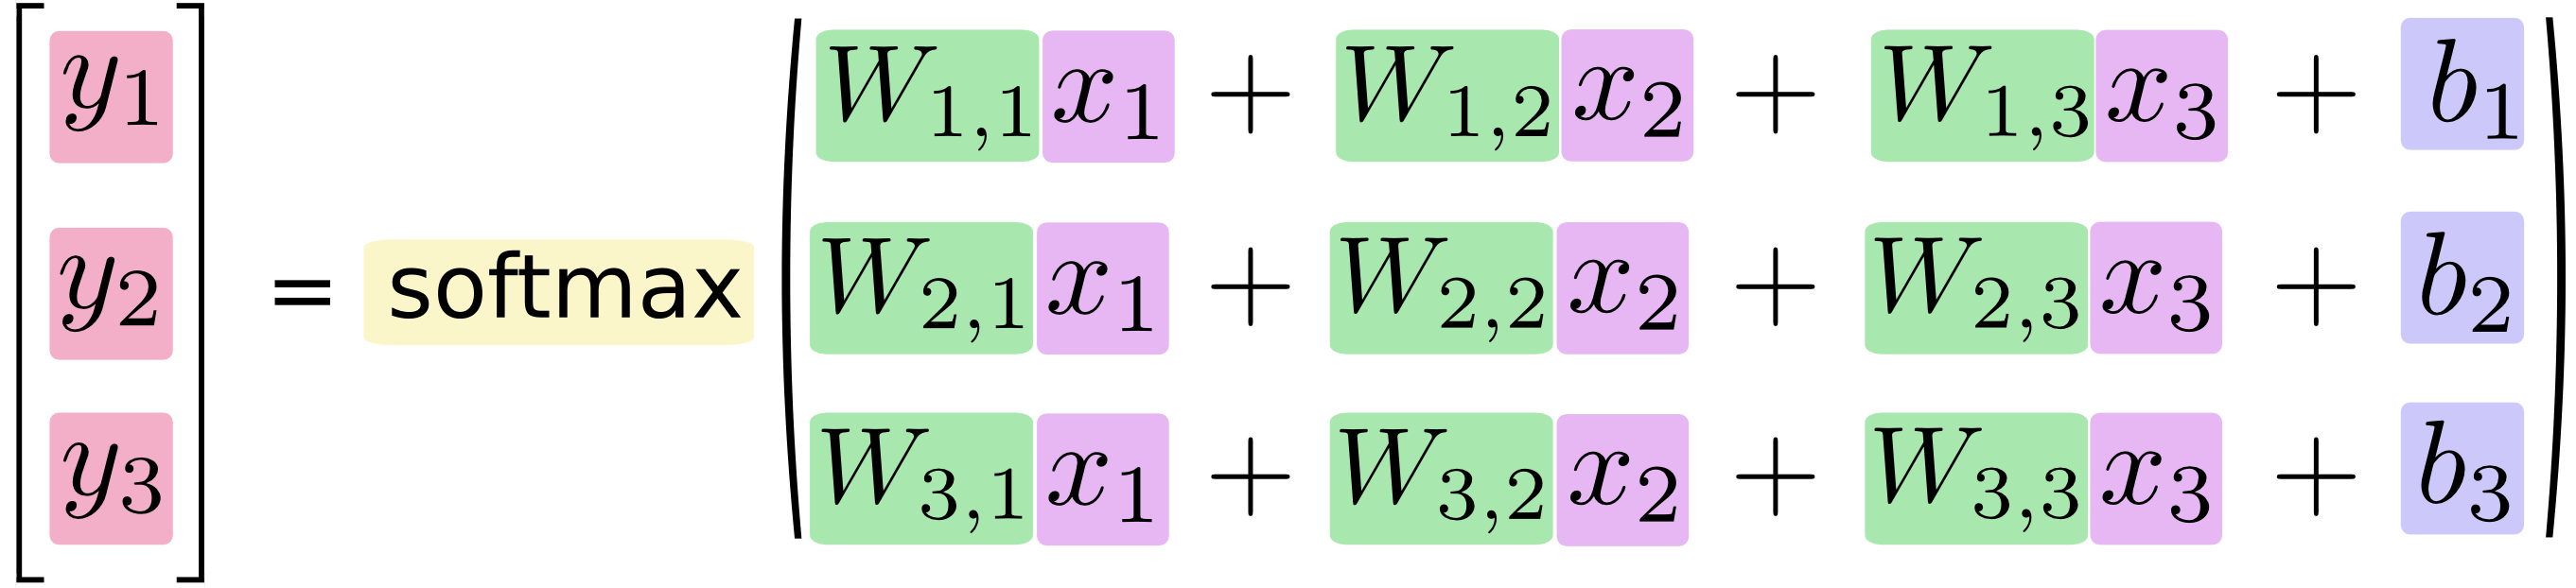
\includegraphics[scale=0.042]{pics/softmax_regression_scalarequation}
			\caption{Softmax Regression mit Skalaren.}
			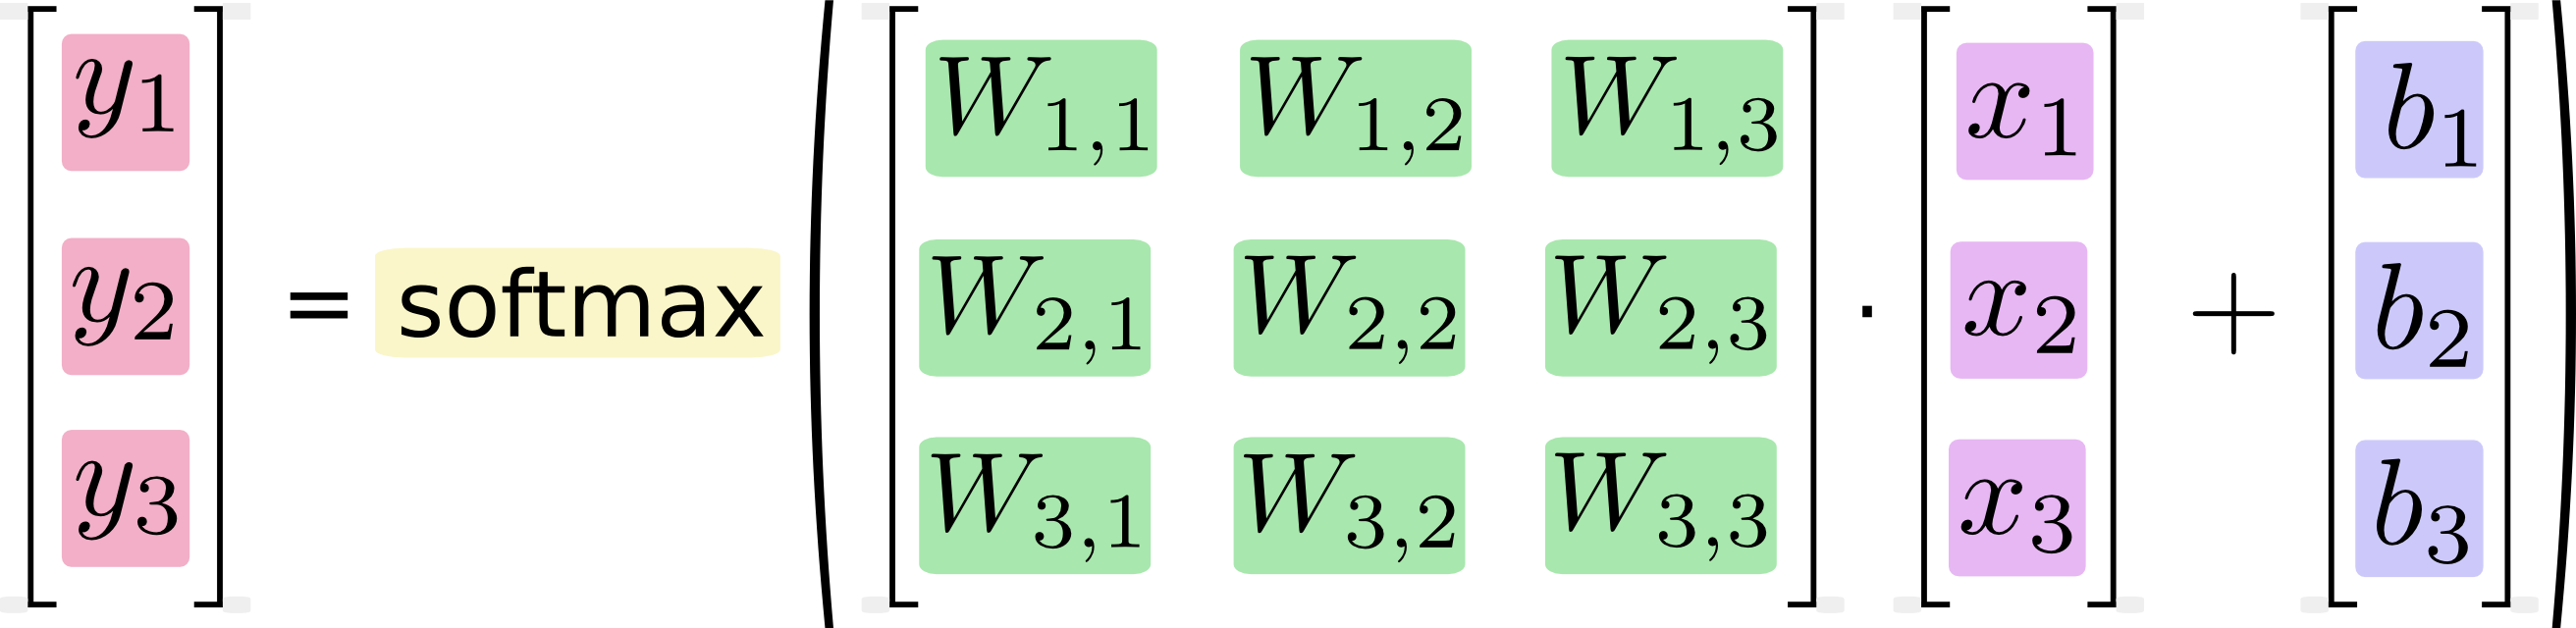
\includegraphics[scale=0.042]{pics/softmax_regression_vectorequation}
			\caption{Softmax Regression mit Matrix-Vektor-Multiplikation.}	
		\end{figure}			
	\end{block}
	
	\framebreak
	
	\begin{block}{Implementierung in TensorFlow -- Modell I}
		\begin{itemize}
			\item Importieren der TensorFlow-Bibliothek
			\begin{lstlisting}
	import tensorflow as tf
			\end{lstlisting}
			\item Definiere Platzhalter für die Inputbilder (Eingabe von beliebig vielen Bildern $B$)
			\begin{lstlisting}
	x = tf.placeholder(tf.float32, [None, 784])
			\end{lstlisting}
			\item \tt{None} $\rightarrow$ Dimension kann beliebigen Wert annehmen
			\item Definieren der trainierbaren Variablen (initialisiert mit Nullen)
			\begin{lstlisting}
	W = tf.Variable(tf.zeros([784, 10]))
	b = tf.Variable(tf.zeros([10]))
			\end{lstlisting}
		\end{itemize}
	\end{block}
	
	\framebreak
	
	\begin{block}{Implementierung in TensorFlow -- Modell II}
		\begin{itemize}
			\item Definition des Modells:
			\begin{lstlisting}
	z = tf.matmul(x, W) + b
	out = tf.nn.softmax(z)
			\end{lstlisting}
			\item Beachte: Matrix-Multiplikation und Vertauschung von $\mathbf{x}$ und $W$
			\item $\mathbf{x}W \in \mathbb{R}^{B \times 10}$ und $\mathbf{b}\in\mathbb{R}^{10}$ $\rightarrow$ Broadcasting
			\item Brauchen als Label einen Platzhalter mit shape $[$None$, 10]$ 
			\begin{lstlisting}
	y = tf.placeholder(tf.float32, [None, 10])
			\end{lstlisting}
		\end{itemize}
	\end{block}
	
	\framebreak
	
	\begin{block}{Implementierung in TensorFlow -- Fehlerfunktion}
		\begin{itemize}
			\item Wann ist das Modell gut? $\rightarrow$ Fehler-/Loss-/Kostenfunktion
			\item Wie weit ist das Modell vom angestrebten Ergebnis entfernt?
			\item Beispiel einer Fehlerfunktion: Kreuzentropie
			\begin{align*}
				H_{\mathbf{y}'}(\mathbf{y}) = -\sum_i y'_i\log(y_i)
			\end{align*}
			mit wahrer Verteilung $\mathbf{y}'$ und Vorhersage $\mathbf{y}$.
			\begin{lstlisting}
	cross_entropy = tf.reduce_mean(-tf.reduce_sum(y * tf.log(out))
			\end{lstlisting}
			\item Numerisch instabil $\dots$ besser:
			\begin{lstlisting}
	cross_entropy = tf.reduce_mean(tf.nn.softmax_entropy_with_logits(y, z))
			\end{lstlisting}
		\end{itemize}
	\end{block}
	
	\framebreak
	
	\begin{block}{Implementierung in Tensorflow -- Training I}
		\begin{itemize}
			\item Fehlerminimierung mittels Backpropagation-Algorithmus
			\item Anpassung der trainierbaren Variablen $W$ und $\mathbf{b}$ mittels Optimierungsverfahren (z.B.
			Gradientenabstieg)
			\begin{lstlisting}
	train_step = tf.train.GradientDescentOptimizer(0.1).minimize(cross_entropy)
			\end{lstlisting}
			\item Gradientenabstieg für Funktion $f\colon\mathbb{R}^n \rightarrow \mathbb{R}$
			\begin{align*}
			\mathbf{x}^{(i+1)} = \mathbf{x}^{(i)} - \alpha^{(i)}\nabla f(\mathbf{x}^{(i)})
			\end{align*}
		\end{itemize}
	\end{block}
	
	\framebreak
	
	\begin{block}{Implementierung in TensorFlow -- Training II}
		\begin{figure}[c]
		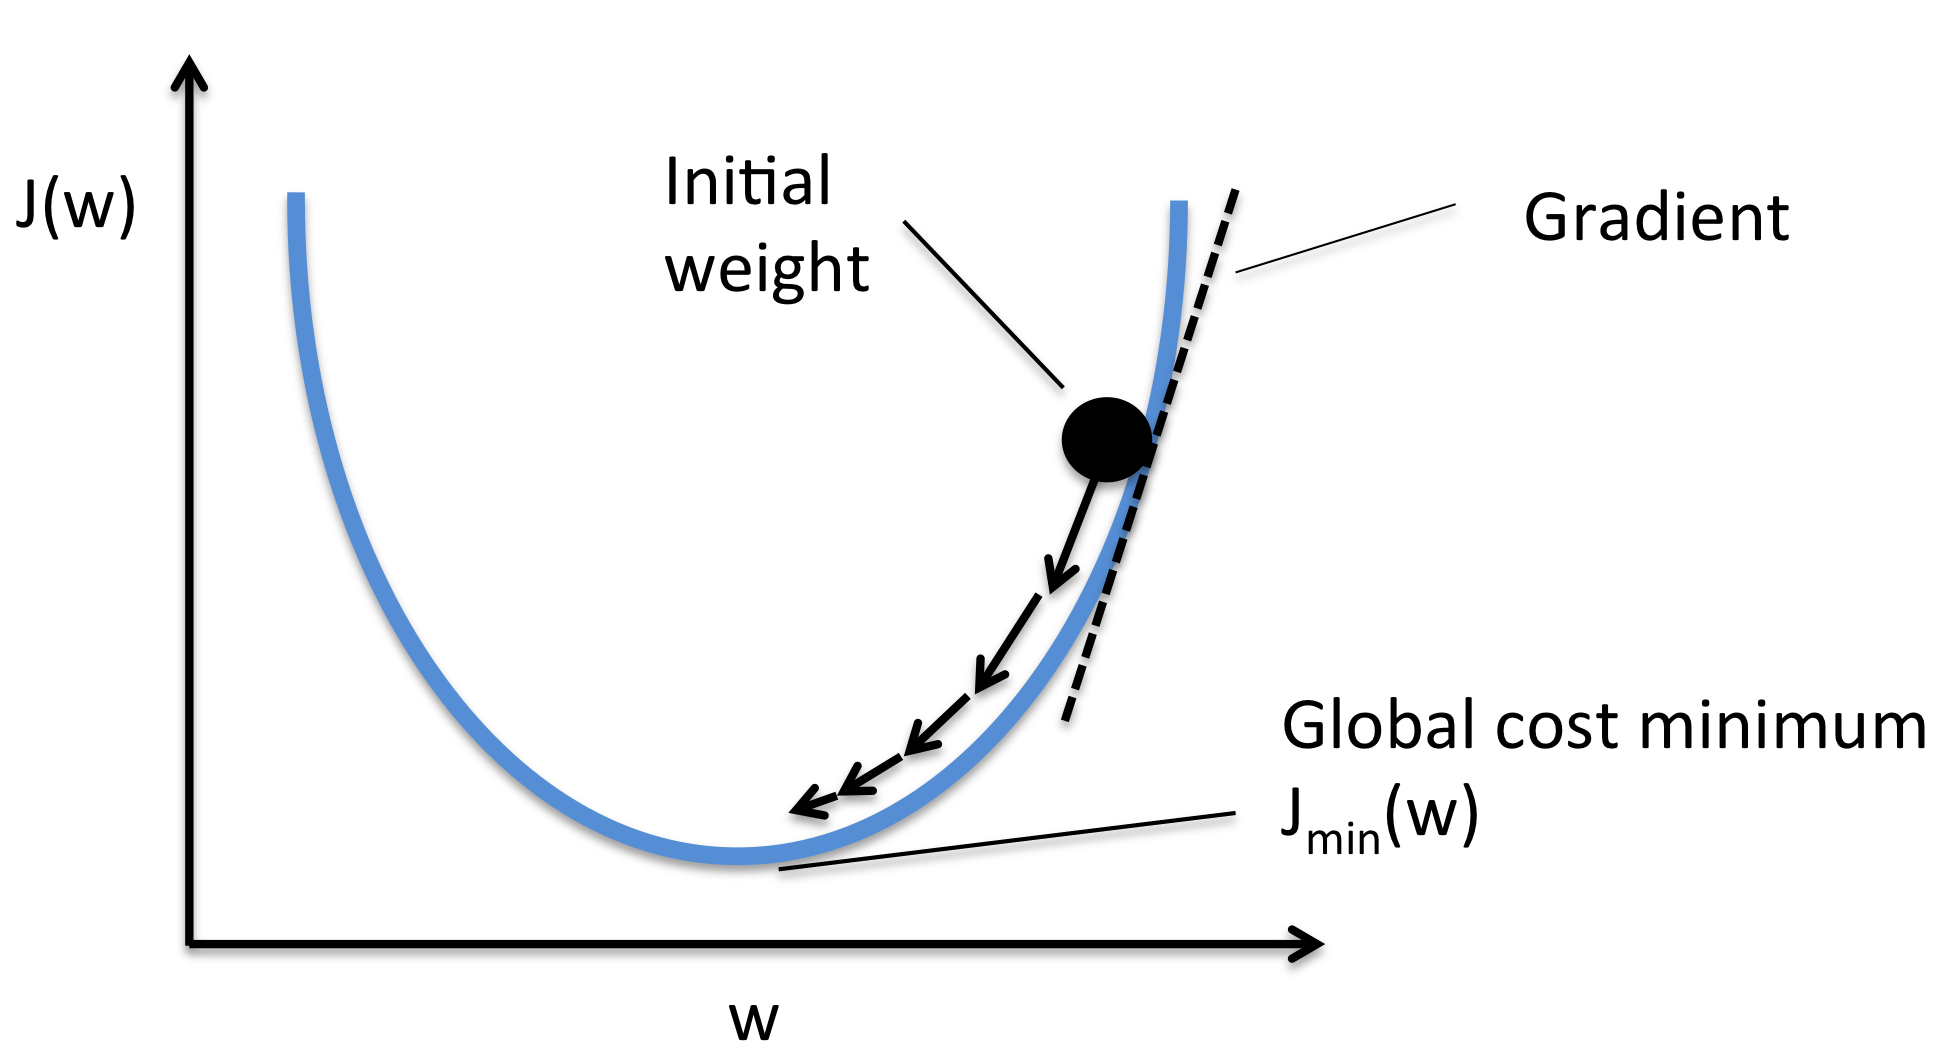
\includegraphics[scale=0.1]{pics/gradient_descent}
		\caption{Gradientenabstiegsverfahren zum Finden lokaler/globaler Minima.}
		%\footnote{\url{https://rasbt.github.io/mlxtend/user_guide/general_concepts/gradient-optimization}}}
		\end{figure}
	\end{block}
	
	\begin{block}{Implementierung in TensorFlow -- Training III}
		\begin{itemize}
			\item Session starten und Variablen initialisieren:
			\begin{lstlisting}
	sess = tf.Session()
	sess.run(tf.global_variables_initializer())
			\end{lstlisting}
			\item Trainingsschritt $5000$ Mal ausführen ($100$ Bilder pro Schritt):
			\begin{lstlisting}
	for _ in range(5000):
		batch_x, batch_y = mnist.train.next_batch(100)
		sess.run(train_step, {x: batch_x, y_:batch_y})
			\end{lstlisting}
			\item Batch: zufällige Menge an Bildern die als Input dienen
		\end{itemize}
	\end{block}
	
	\framebreak
	
	\begin{block}{Implementierung in TensorFlow -- Evaluierung I}
		\begin{itemize}
			\item Wie gut arbeitet das Modell? 
			\item $\arg\max$ einer Funktion $f$ mit Definitionsbereich $D$:
			\begin{align*}
				x_{\max} = \arg\max_{x\in D} f(x)\Leftrightarrow f(x_{\max}) = \max_{x\in D}f(x)
			\end{align*}
			\item Bestimme das wahrscheinlichste Label und prüfe es auf Richtigkeit
		
			\begin{lstlisting}
	correct_prediction = tf.equal(tf.argmax(output, 1), tf.argmax(y, 1))
			\end{lstlisting}
		\end{itemize}
	\end{block}
	
	\framebreak
	
	\begin{block}{Implementierung in TensorFlow -- Evaluierung II}
		\begin{itemize}
			\item Bestimme die Genauigkeit des Modells:
			\begin{lstlisting}
	accuracy = tf.reduce_mean(tf.to_float(correct_prediction))
			\end{lstlisting}
			\item Ausgabe der Genauigkeit auf den Testdaten (\textasciitilde$92\%$):
			\begin{lstlisting}
	print(sess.run(accuracy, {x: mnist.test.images, y: mnist.test.labels}))
			\end{lstlisting}
			\item CNNs können über $99\%$ Genauigkeit liefern, bis zu $99,7\%$ als bester Referenzwert.
		\end{itemize}
	\end{block}
\end{frame}
\fi

\end{document}

